% !TeX root = main.tex


\chapter{State of the Art}
\label{chap:2}
Chapter \ref{chap:2} introduces the theoretic baselines for data acquisition, data metrics as well as standardized data formats in which to save metadata. Topics to consider when starting the Sensor Health Monitoring process are mainly that of providing a structured overview of the Sensor Metadata which in itself consists of many layers as a dynamically generated set of metadata is desired. This is motivated by the desire to represent changing Data Acquisitioning (DAQ) System configuration changes in the metadata system. Consideration is given to the SOIL data model and its' ability to handle the many demands that are expected of sensor data management. \cite{behrens_domain-specific_2021}
The second major part to consider is that of physical cross relations and deep checks which are an experimental mode of checking for inconsistencies among the data. Major research and implementation work goes into developing a dynamic model that is generated from the data and then checks back upon the data for possible discrepancies. This approach is chosen as it is estimated to be the most structured approach for a first prototype.


\section{The ISTAR}
\label{chap:meet_the_istar}
%Todone: explain the istar system, DAQ and possible error locations in the complex system
The data itself is the essence of this work. The data used in this work is recorded in the ISTAR aircraft, a Falcon 2000LX. Since 2019 it is part of the DLR's research aicraft fleet (see Figure \ref{fig:dlr_fleet}). The ISTAR possesses a large databus with over 40,000 parameters that are essential to transmit system info of singular aircraft components to the Flight Management Computer (FMC) and other recipients within the aircraft. These parameters consist of Primary aircraft data such as sensor measurements but a majority of the parameters consists of secondary derived data and status bits that are present in various SI-units and imperial aerospace units as well as data formats ranging from Boolean values to integers, floats and strings. The special part of the ISTAR's customization lies within its recording of aircraft bus parameters which allows to retroactively analyze flights. Facilitated by a DAQ that records the main aircraft bus, an additional inertial positioning unit, experimental aeroelastic sensors and the noseboom over 400 sensor parameters are recorded per flight.

\begin{figure}
    \centering
    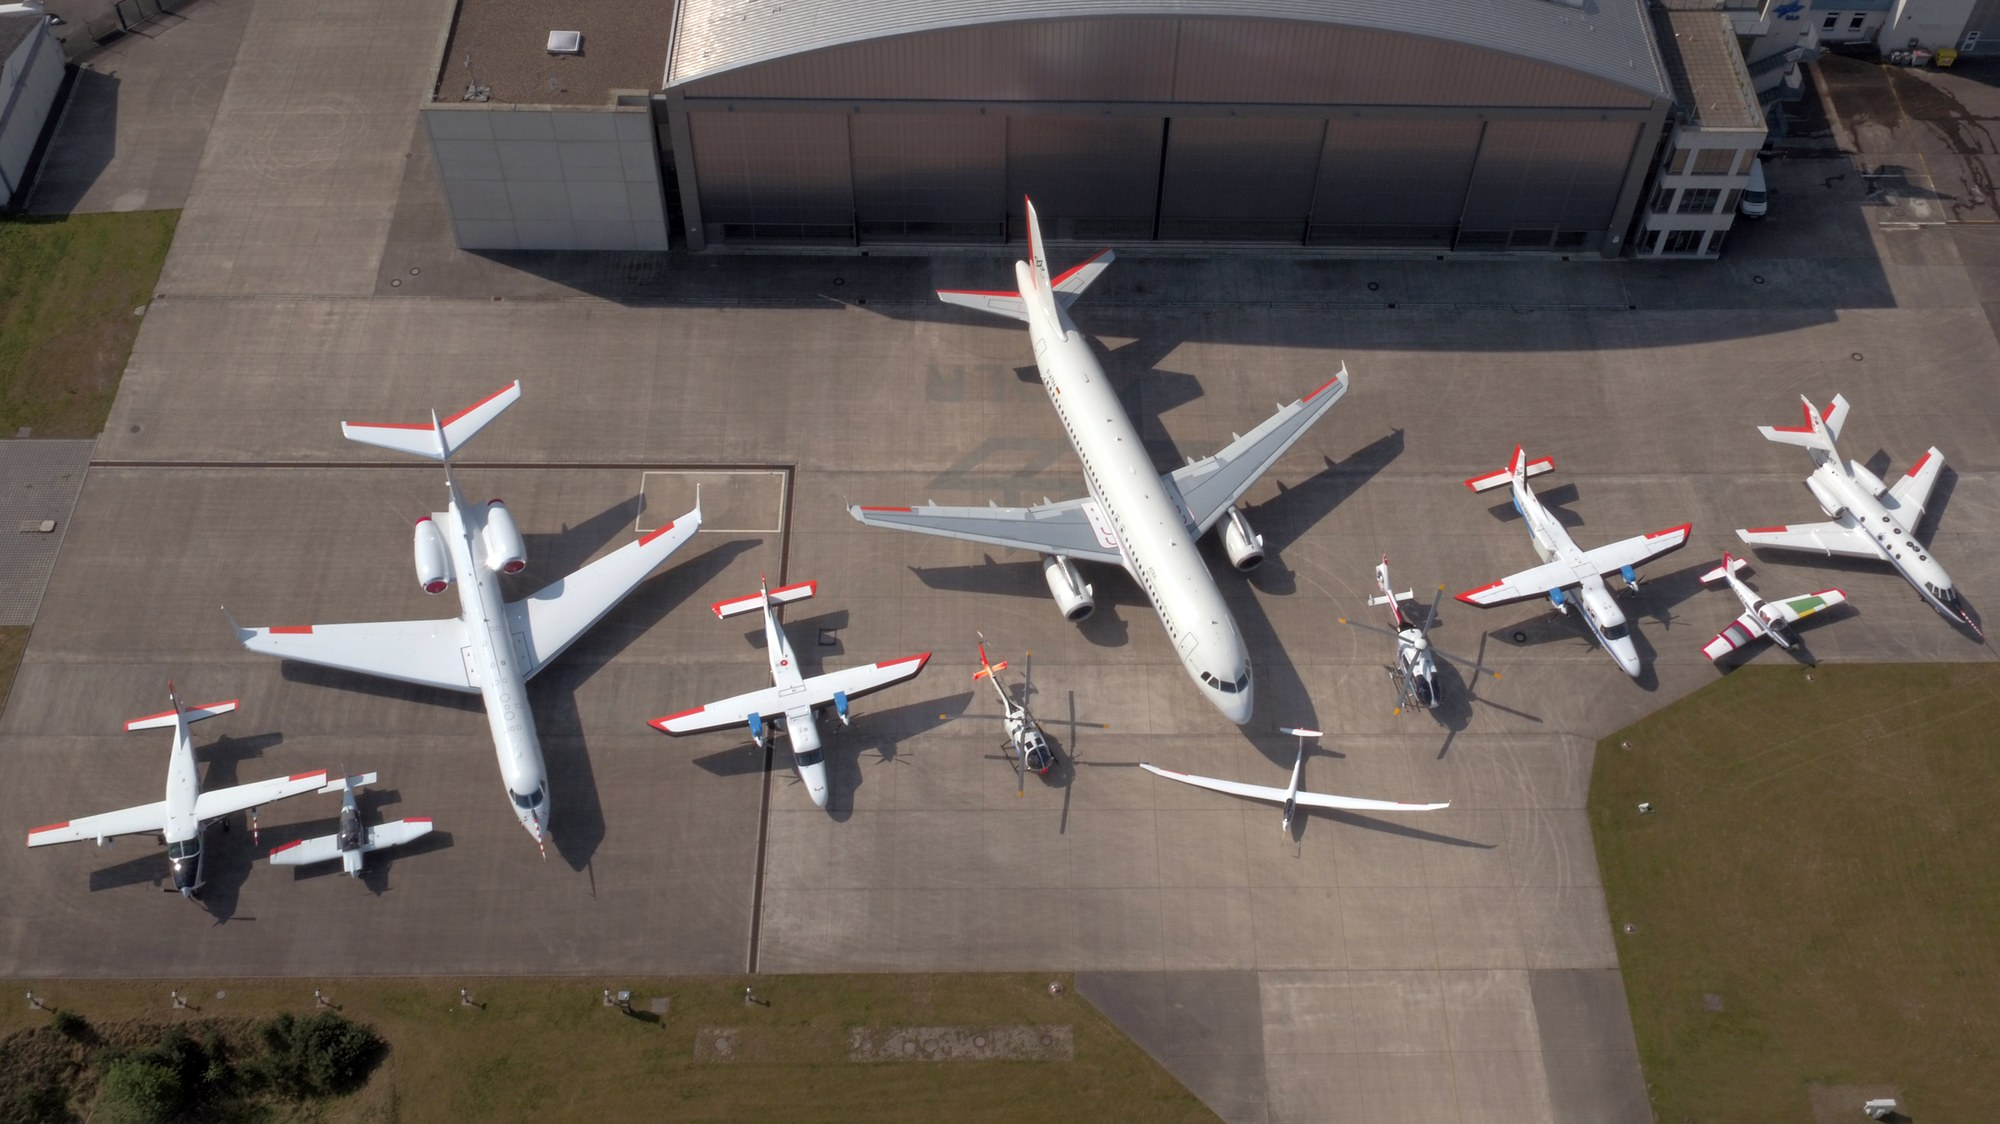
\includegraphics[width=0.7\textwidth]{dlr_fleet.jpeg}
    \caption{The DLR's research aircraft fleet \cite{dlr_dlr-fleet_2018} lined up for a photo shoot at the DLR Brunswick site}
    \label{fig:dlr_fleet}
\end{figure}

The ISTAR will be examined since its measurement data for Digital Twin applications needs to be certified in respect to its data quality. The aircraft system itself is tested and sensor errors are displayed to the pilots during the flight. However, there is no way to record these error messages and modify the fault detection algorithms to the custom experimental sensors. In addition, the DAQ hardware is certified to be safe within the aircraft (e.g. electromagnetic compatibility, avoiding spontaneous inflammation) to refrain from detrimenting flight conditions but it is not configured to also provide data reliably with a standard reliability of $10^{-6}$. This further motivates the desire for an open SHM to further data knowledge and insights.

\subsection{System overview}

The ISTAR's data acquisitioning system (DAQ) is the hub to record and centralize all aircraft data and will be regarded as the focal element of this work. As previously mentioned the DAQ is not tested up-to aircraft standards. Because fault detection is shown in the cockpit during the flight but is not recorded in the DAQ it is necessary to implement such a fault detection. The data flow within the aircraft is complex and nested. The DAQ firstly taps into the main aircraft bus that is within the Avionics Standard Communications Bus, Version D (ASCB-D) as well as the aeroelastic sensors (strain gauges and accelerometers), the Nose-Boom (instrumentation to measure undisturbed airflow) and a highly precise additionally installed combined Inertial-Navigation-System (IMS) and Geodetical Navigation Satellite System (GNSS). As any other aircraft, the necessity of various reference systems is necessary. Generally, the geodetic, aerodynamic, airframe-fixed and track-fixed coordinates system are used \cite{brockhaus_flugregelung_2011}. These compensate various effects and facilitate interpretation of various primary and secondary parameter values

\subsection{Sensor to DAQ}
% pitot tube, sampling, to DAQ

In the following, an exemplary flow of information from a Pitot Tube is described, illuminating the various facets and trade-offs that need to be made along the way to the main aircraft bus and then the DAQ. In Figure \ref{fig:istar_wires} the exemplary data flow for a single sensor to the DAQ is shown. The Pitot Tube (PT) measuring a dynamic pressure is chosen for this exemplary case.
\begin{figure}[h]
    \centering
    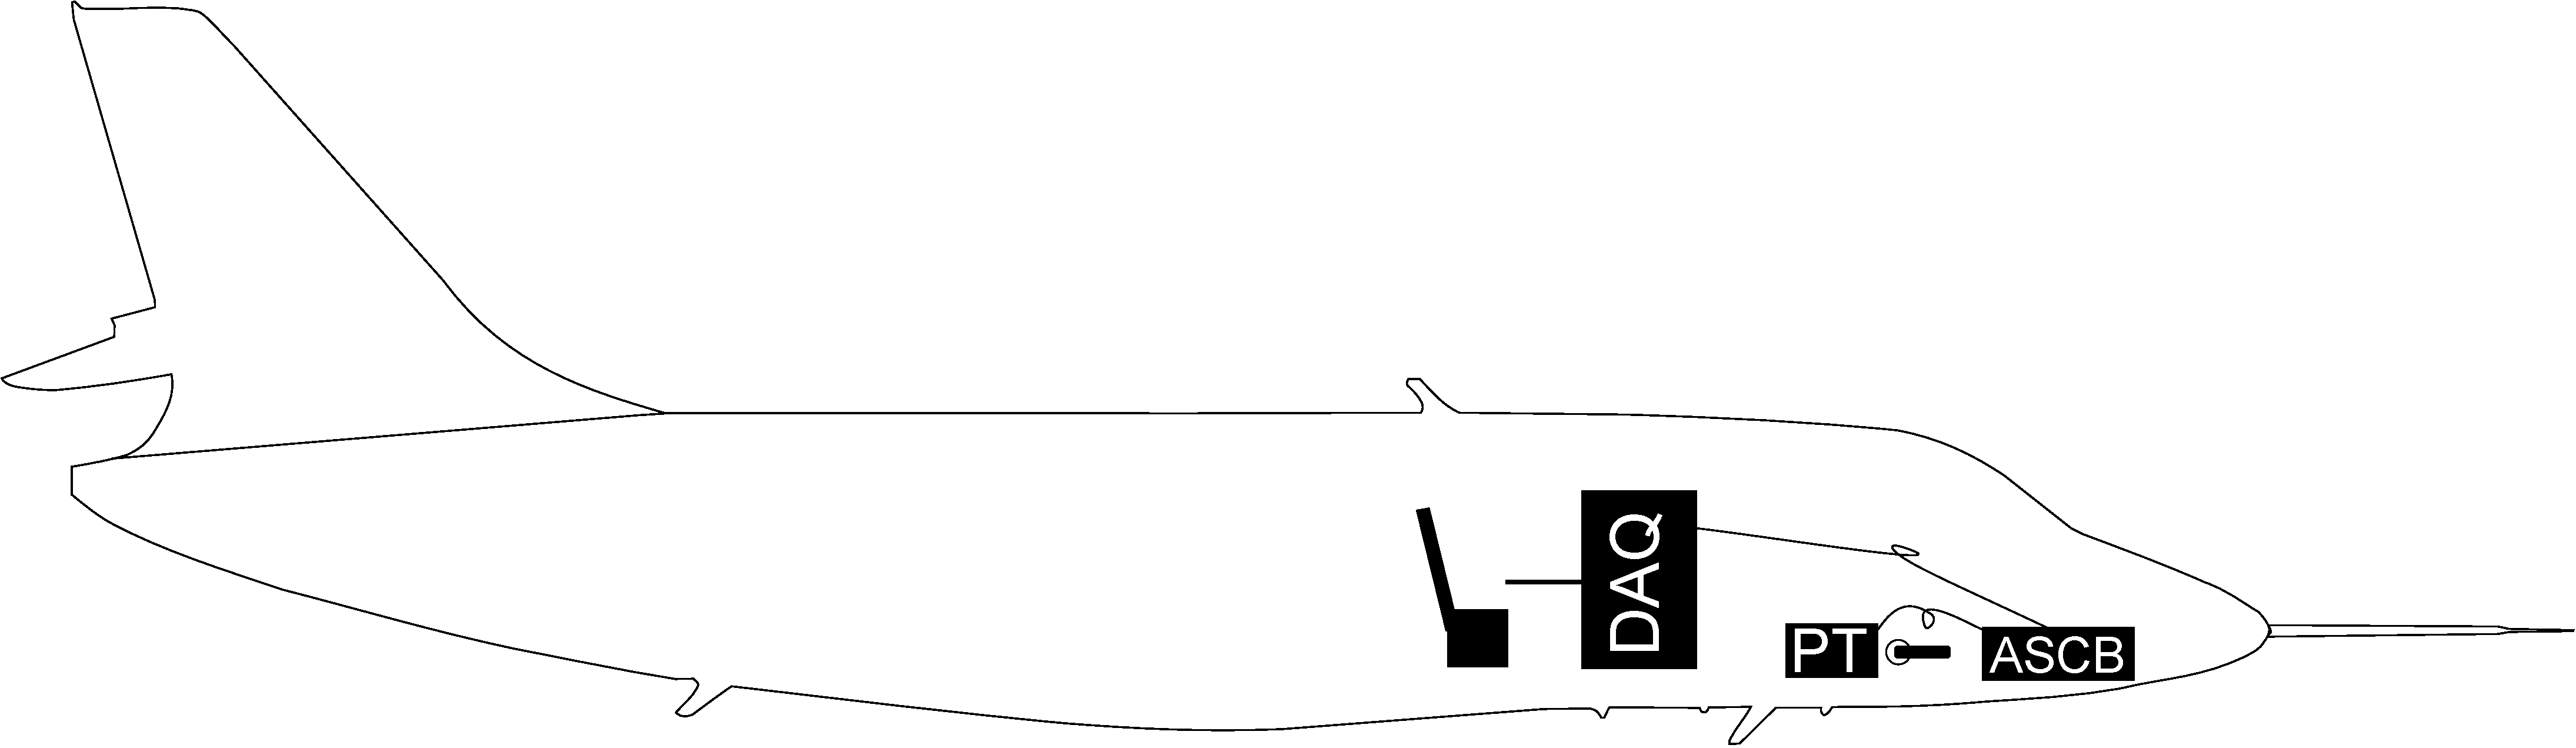
\includegraphics[width=\textwidth]{istar_wires}
    \caption[The ISTAR crosssection displaying sensor information flow]{The ISTAR data flow with a Pitot Tube (PT) sending its data to the ASCB-D bus via the Air Data System (not shown) and then to the DAQ. Each entity of the flow applies its own sampling of data.}
    \label{fig:istar_wires}
\end{figure}


% todone: show data flow steps by matthew. Exemplary data flow for sensors including sampling rate and  reliability
The Flight Test Data by the ISTAR gets recorded by a base DAQ system by IMC co. This base contains inputs from the main aircraft data bus, the experimental nose boom, experimental strain gauges and acceleration sensors as well as an experimental Inertial Measuring Unit (IMU) combined with a GNSS-System. In addition, complementary DAQs are added to fulfill given experiment requirements. In regard to system complexity it is notable that the main aircraft bus data originates from various sources, ranging from air data that gets measured by a sensor working on an electric current which then gets transformed by an Analog Digital Converter (ADC) into a digital, discretized signal which then gets fed into the main aircraft bus system. Such a signal would then get transmitted to the IMC DAQ, making troubleshooting a multifaceted problem within this system due to the multiple points of failure.

\subsection{State to Sensor}
%todo: state to sensor klingt scheiße. Neue Überschrift nötig
Within the following, some consideration is given to the inherent flaws lying in the actual measurement of state values. The Pitot Tube system from Figure \ref{fig:istar_wires} is examined in detail in Figure \ref{fig:signal_processing} showing the choices, experimenters need to make and the tradeoffs they inherit. An example is the sampling rate. Sampling at higher rates delivers much more precise results. It however also generates proportionally more data. It is then necessary to determine a sampling rate that is apt for each experiment. The Nyquist-Shannon sampling theorem is an aid in deciding the desired frequency since it establishes that the sampling frequency can only detect signals that are less than half its frequency as shown in Equation \ref{eq:nyquistshannon}. \cite{smith_scientist_1999}
\begin{equation}
    f_{sampling} > 2 \cdot f_{max}
    \label{eq:nyquistshannon}
\end{equation}
For context in this work, the ASCB-D has the tradeoff that it resamples all aircraft signals to 20Hz which in turn leads to some information loss with some signals being downsampled and some being oversampled. For most applications the Sampling of 20Hz is satisfactory although a resampling of any data inherently leads to information loss and is thus not desirable in most cases. This makes potentially noisy sensors output the same value twice in a row since the DAQ hasn't yet received the new sensor data and outputs the same value multiple times in a row. Even sensors with a high noise ratio such as the fine part of a GNSS latitude signal may sometimes output the same value twice in a row which is highly unlikely to happen on a statistical basis. Since this occurs quite often the question arises if the actual sampling may be lower or higher than the actual data. Perhaps it is then justified to resample some data to reduce oversampling in order to increase the data quality mitigating the changes made by the systems in and around sensor and DAQ.

For Illustration, an exemplary time-, and value-sampling of a Pitot Tube is shown.
\begin{figure}[!h]
    \centering
    \begin{subfigure}{\textwidth}
        \centering
        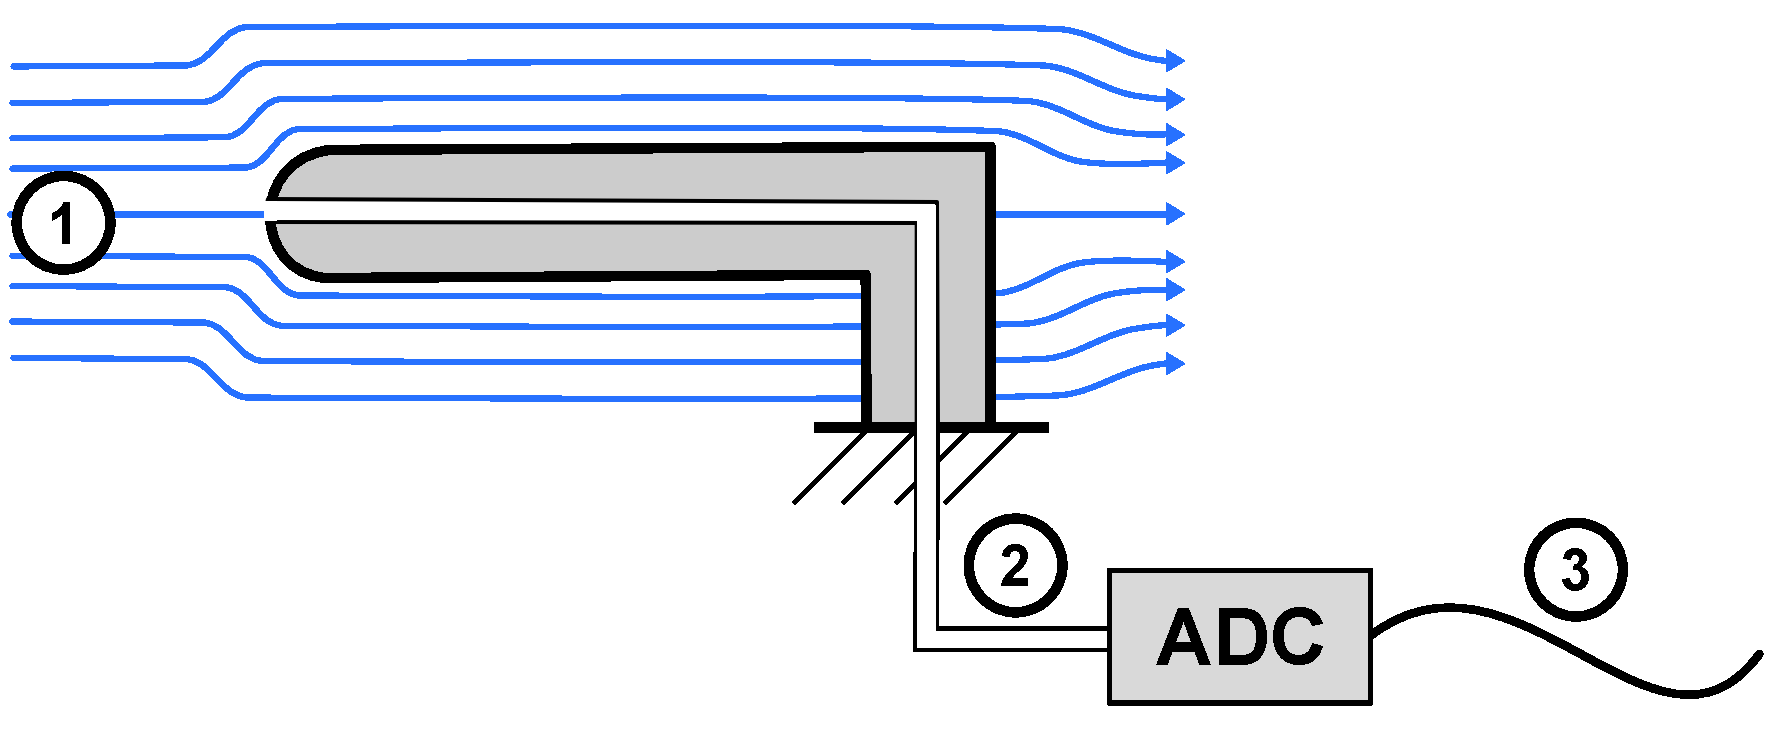
\includegraphics[width=0.8\textwidth]{03_figures/signal_recording}
        \caption[Exemplary pitot tube for visualizing sensor error]{A pitot tube setup for measuring dynamic pressure in order to measure aircraft velocity. Three spots are marked in which the state signal is skewed in a significant way.}
        \label{fig:signal_processing_setup}
    \end{subfigure}
    \begin{subfigure}{\textwidth}
        \centering
        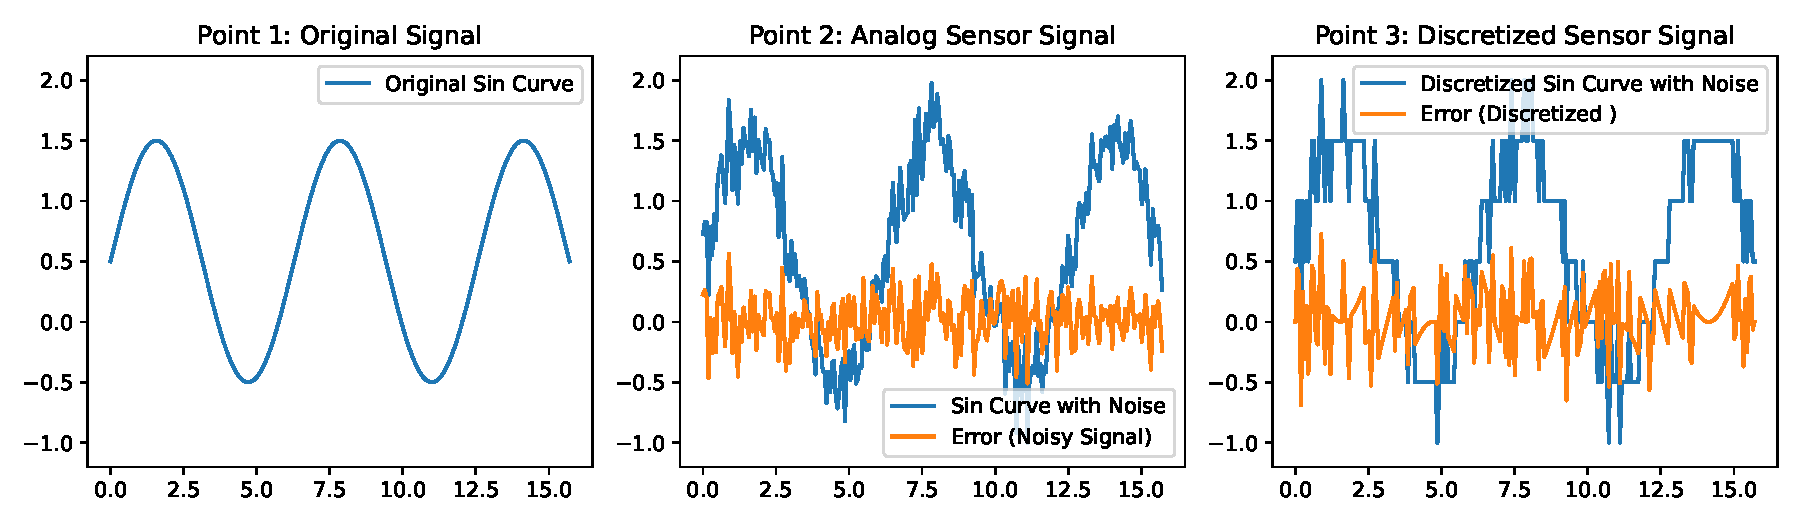
\includegraphics[width=\textwidth]{03_figures/python_functions/images/signal_processing_plots}
        \caption[Pitot Tube signal visualization with inherent errors]{Original signal transformed into measured and discretized signal. The signal transformation at each step is shown together with the error occurring at each step}
        \label{fig:signal_processing_plots}
    \end{subfigure}
    \caption[Exemplary signal processing flow for a pitot tube]{An illustration of random signal errors for a pitot tube. The Figure contains the undisturbed state variable (1), the unmodified measurement by the analog sensor (2) and the digitized, discretized sensor (3) values. In Figure \ref{fig:signal_processing_plots} the modified signal is shown in blue with the error in orange.}
    \label{fig:signal_processing}
\end{figure}

The undisturbed system state at point 1 gets measured by a sensor and is transformed into the analog, measured signal at point 2 with the error being represented by the orange plot. An ADC is used in the next step of the signals journey and discretizes the time by sampling the signal to a given frequency and a discrete value given by a given resolution. Having been digitized at point 3 the signal error subsequently grows even further. Other error mechanisms that occur randomly (stochastic) include but are not limited to sensor drift as well as random noise. In the following, qualifiers and descriptors are introduced to quantify these qualities.




\newpage


\section{Definitions}
Motivating this section is the desire to understand the fundamental error mechanism. Definition for errors are adopted from \textcite{isermann_fault-diagnosis_2006} defined in table \ref{tab:system_props_isermann}, the de-facto standard of Fault Diagnosis descriptions within the automation domain.

\subsection{Errors}

To find and detect errors it is firstly important to understand them. Within Table \ref{tab:system_props_isermann} errors are described as the difference between measurement and actual value as seen in Figure \ref{fig:basic_error}. Sensor are used to measure physical states in the world. But how precise do they measure? No sensor is without error, an inevitable property accompanying every sensor application. In the following, sensor errors are classified into categories upon which an understanding about data quality can be built that then can describe the data quality of the ISTAR datasets.
\begin{table}[h]
    \centering
    \caption[Error Type Overview]{A general overview over the three different Error Types. Systemic errors are errors which are predictable and can be modeled mathematically. To compensate systemic errors a calibration process can be applied which removes the entire systemic error. The second error type is the random error which occurs constantly and behaves unpredictably. Random Errors are generally also understood as white noise. Lastly, the failure forms the final type of error type. It signifies through relatively rare occurrence but a then fatal failure of the data source. A solution for random errors is redundancy of sensors and the mixing of single sensor values.  \cite{hartmann_flugfuhrung_2022}}
    \begin{tabular}{@{}llll@{}}
        \toprule
        Error Type     & Appearance    & Occurrence & Compensation \\ \midrule
        Systemic Error & Deterministic & Permanent  & Calibration  \\
        Random Error   & Stochastic    & Permanent  & Filtering    \\
        Failure        & Stochastic    & Occasional & Mixing       \\ \bottomrule
    \end{tabular}
    \label{tab:error_types}
\end{table}
\newpage

Identifying sensor errors is the goal of this thesis. As described in Figure \ref{fig:basic_error} the error can be imagined as a disturbance added upon the original sensor value. Which then results in a skewed sensor measurement.

In Table \ref{tab:error_types} sensor errors are divided into 3 subcategories which are classified by their appearance representing their manageability. Deterministic Errors can be easily compensated since they are reproduceable. Stochastic Errors however are non-deterministic. Figure \ref{fig:sensor_errors_systemic} gives an overview over systemic errors which generally are compensated by using calibration mechanisms in practical applications. The sensors within this work are assumed to be calibrated so this property is solely mentioned for completeness. However, perhaps some new understandings may be gained after a full SHM routine has been implemented since accuracy of calibration specifications is only as accurate as previously specified by the operator.

\begin{figure}[h]
    \centering
    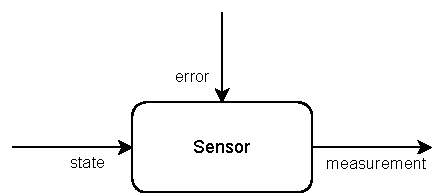
\includegraphics[width=0.5\textwidth]{basic_error}
    \caption{A sensor measurement is always the result of the actual true value plus a measuring error.}
    \label{fig:basic_error}
\end{figure}

%todo: backlog: fehlerarten besser erklären
Errors that also occur continuously are random errors that are however unpredictable in their behavior. To compensate those errors, filtering can be applied by e.g., high- or lowpassfiltering. The final error type mentioned in Table \ref{tab:error_types} is sensor failure. This is characterised as a spontaneous event in which the sensor information stream is completely interrupted.

\begin{figure}[h]
    \centering
    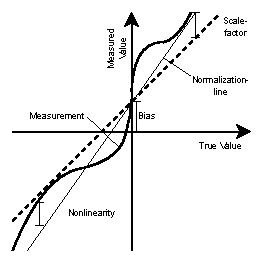
\includegraphics[width=0.4\textwidth]{sensor_errors_systemic}
    \caption[Systemic Sensor Errors]{The types of systemic sensor errors introduced in Table \ref{tab:error_types} are shown by plotting the measured value over the true value. \cite{hartmann_flugfuhrung_2022, din_fundamentals_1995} }
    \label{fig:sensor_errors_systemic}
\end{figure}
% todo: im allgemeinen noch mehr zu abbildungen erzählen. mehr motivieren QEC?
Now the question poses if errors can be pinpointed to their origin from where such errors arise. Generally, single sensors carry inherent errors such as clogged static ports (spontaneous hysteresis) or sensor drift (spontaneous bias) but errors also occur within the complex aircraft system architecture itself. An exemplary process step is the Analog to Digital Conversion. Sensor outputs are primarily analog but are then digitized in order to get transported by the aircraft data bus. This process is accomplished using an Analog Digital Converter (ADC), effectively eliminating information from the system. The full process is shown in Figure \ref{fig:signal_processing}.

\subsection{Data Quality}
% todo: kommentar einfügen: Oder ganz generell: Um erkennen zu können ob das gemessene Signal richtig sein können muss das System wissen was es misst. Diese Information muss in maschinenlesbarer Form vorliegen
Foundation for this work lies within a common understanding of its results. Standardized qualifiers are found within control theory \cite{isermann_fault-diagnosis_2011} as well as GNSS applications \cite{teunissen_springer_2017}. Standardization is also found within the ISO-Database. However, when beginning to describe data quality within metadata, the issue of metadata quality itself also arises. In the following, a brief overview is given over descriptors and their qualities based on norms.

\paragraph{A general introduction to Semantics}
Semantics is a broad term due to its common use. One definition that has found some acceptance is the definition by Metzlers Lexikon which relies on theories by Blackburn and Kutschera \cite{shoemaker_spreading_1987,kutschera_sprachphilosophie_1975}. The following paragraph contains a small explanatory parenthesis to motivate the term Semantics and its parent term being the field of semiotics. Semiology (greek:\textgreek{σημεῖον},semeion:sign) describes the theory of signs and their usage as described in Figure \ref{fig:semiotics}. It is divided into the areas of semantics, syntactics and pragmatics in which syntactics are defined as the internal structure of signs within sign systems. In the next step pragmatics are defined as the theory of sign usage effectively thinking about how interaction with signs works. Finally, semantics define the relationship between signs and described objects. They work by allocating a structure or model to a predefined expression in the way a metadata model uses standardized descriptors to represent a meaning in the real world.

\begin{figure}[h]
    \centering
    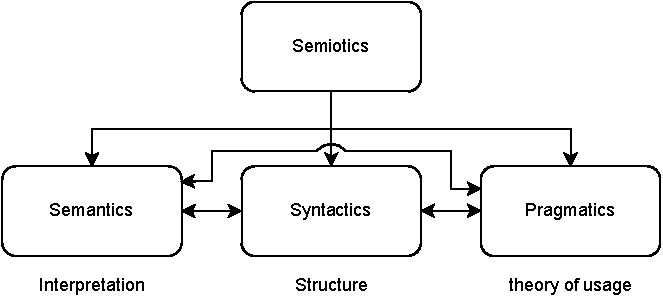
\includegraphics[width=.7\textwidth]{03_figures/semiotics.pdf}
    \caption[A semiology overview]{Semiology, according to \textcite{kutschera_sprachphilosophie_1975} and \textcite{shoemaker_spreading_1987} contains three subfields of semantics, syntactics and pragmatics which form the cornerstones of common sign usage.}
    \label{fig:semiotics}
\end{figure}

This gets developed further within ISO 8000-8: Data Quality \cite{iso_data_2015}, concluding that syntactic qualities define the structure of the content language and semantic qualities define the structure of the content itself to allow verifying information. Whereas pragmatic qualities describe the use that can be extracted from the content itself hence allowing validation.

Contextually, the metadata syntax of this work will be in a JSON-format. The used semantics will be standardized to use the SOIL (SensOr Interfacing Language) structure and pragmatics will be quantified by the validity of the actual metadata. Moving on from these fundamental concepts, the pragmatic data qualities will be defined in the following.

\paragraph{Metadata descriptors}

Unambiguous terms are needed to provide clear and concise information within the sensor health monitoring data structure. This is especially important to create a common base of understanding. In the following, industry standards and definitions for data metrics are summarized.

Definitions based on a control theory background are shown in table \ref{tab:system_props_isermann}. These have been agreed upon in discussion with VDI and VDE committees as well as the Reliability, Availability and Maintainability (RAM) dictionary. \cite{isermann_trends_1997,din_fault_1977}

These terms are divided into the contextual categories of primarily defining signal and state descriptors. Next up are functions for fault processing followed by model attributes that are employed to compare them to the actual system. System properties can then be inferred by leveraging the previous descriptors for states, functions and models. Illustrating the fault detection process, Figure \ref{fig:basic_error_filter} shows the method generating a residual which in turn enables interpretation of said residual which may contain information to isolate and identify the error.


\begin{figure}[ht]
    \centering
    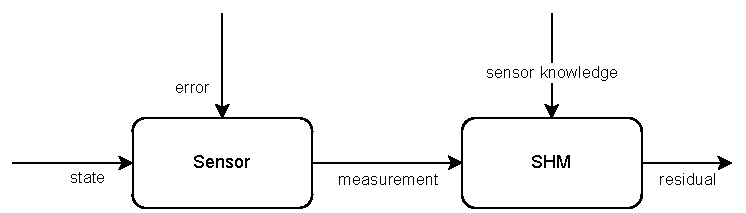
\includegraphics[width=0.5\textwidth]{basic_error_filter}
    \caption[Model-Based Sensor Monitoring]{Comparing the sensor signal to a model-based value yields a residual which can be used to quantify the sensor error.}
    \label{fig:basic_error_filter}
\end{figure}




Further definitions are also employed by the Federal Aviation Administration (FAA) adding integrity as an attribute for GNSS systems that is a quantifier for trust that can be put into the system's measurements. Providing users with warnings when measurements are expected to be unreliable. \cite[B.1.5, B.1.10]{federal_aviation_administration_federal_2008}

\begin{figure}[h]
    \centering
    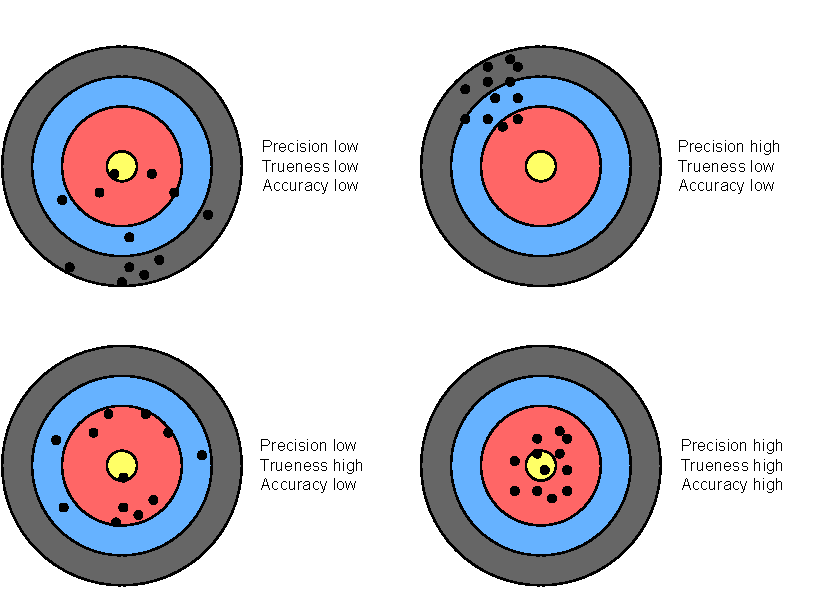
\includegraphics[width=0.7\textwidth]{dart_boards}
    \caption[Data Quality Dartboards]{Dart boards displaying the Precision (as $\sigma$), Trueness (as $\mu$) and Accuracy as the cumulative sensor quality \cite{iso_accuracy_1997}}
    \label{fig:dart_boards}
\end{figure}

Following the GNSS domain, the terms accuracy and precision are important measures for quantifying results. For representation, a dart board is illustrated in Figure \ref{fig:dart_boards}. It is then important to distinguish that good accuracy is the result of good precision as well as a good trueness. A mathematical description for the precision could be the standard deviation and the deviation of mean and actual value as the trueness. \cite{iso_accuracy_1997}\cite[S.33ff.]{smith_scientist_1999}




\begin{table}
    \centering
    \caption{Terminology for system properties  \cite{isermann_fault-diagnosis_2011}}
    \begin{tabular}{@{}ll@{}}
        \toprule
        Descriptor            & Description                                                                               \\ \midrule
        States and Signals    &                                                                                           \\ \midrule
        fault                 & unpermitted deviation of one subset of the system                                         \\
        failure               & permanent interruption                                                                    \\
        malfunction           & intermittent regularity                                                                   \\
        disturbance           & unknown, uncontrolled input                                                               \\
        perturbation          & input, leading to temporary departure from steady state                                   \\
        error                 & deviation between measurement and true value                                              \\              & $y_e = \bar{y} -y$                               \\
        residual             & deviation between measurements and model-based calculations                                                                                           \\       & $\hat{y} = \bar{y} -y_m$                                                              \\ \bottomrule
        Functions       &                         \\ \midrule
        fault detection  & determination fault presence                                  \\
        fault isolation       & Determination fault properties: kind, location, time of detection                                       \\
        fault identification            & determination of size and time-variant behavior of fault                               \\
        fault diagnosis           & includes fault detection, isolation, identification                         \\
        monitoring            & real-time determination of possible physical conditions and                          \\                & recognition, indication of behavioral anomalies                                                                                           \\
        supervision          & monitoring and taking actions to maintain operation during faults                                        \\
        protection           & means by which potentially dangerous behaviors are suppressed if                                          \\            & possible or how consequences are avoided                                       \\ \bottomrule
        Models &           \\ \midrule
        quantitative     & describe system in quantitative mathematical terms                                                                                           \\
        qualitative           & describe system in causalities and if-then rules \\
        diagnostic                & link specific inputs (symptoms) to outputs (faults)             \\
        analytical redundancy          & determine a quantity in an additional way by using a mathematical process model                                                              \\ \bottomrule
        System Properties             &                                                                           \\ \midrule
        reliability                 & ability to perform a function, measure $MTTF$, with $\lambda$ as rate of failure per hour                                                                            \\
        safety        & ability of a system not to cause danger to persons, equipment and environment                                                                      \\
        availability          & $A=\frac{MTTF}{MTTF + MTTR}$                                                                       \\ \bottomrule

        $\lambda$          & rate of failure                                                                       \\
        $\mu$          & rate of repair                                                                       \\
        MTTF=1/\lambda          & Mean time to failure                                                                       \\
        MTTR = 1/\mu          & mean time to repair                                                                       \\ \bottomrule
    \end{tabular}
    \label{tab:system_props_isermann}
\end{table}

%\subsection{Integrity, Reliability and Validity based on GNSS or NORMS von Lars}
%Data according to ISO 8000 cite [ISO22]
%iso5725: -accuracy(validity)+precision(reliability)
%Also see precision and accuracy definition


%Validation: Black Box Testing. Results match expectations Verification: White Box Testing. Establish algorithm's truth

\newpage


\section{SHM Algorithms}
%todo: capitalize figure-->Figure for all occurrences
Building now upon a solid foundation of descriptors, some previously implemented systems dealing with monitoring and supervision tasks are reviewed. The superset of these monitoring systems is generally described as Failure Mode and Effect Analysis (FMEA). In the following, some FMEA implementations are reviewed. Theoretic fundamentals for this works' actual implementation are then shown, checking sensor values against limits and then correlating sensor values with each other.


For the SHM process three distinct steps are proposed to filter out malfunctions by severity and to order the process flow. This entire flow is shown in Figure \ref{fig:SHM_simplified} displaying the proposed essential steps of the SHM. The core of the work is the data processing represented by the gear icon. A core problem of this work is finding a standardized way to transfer information between steps. In order to solve this a metadata model will have to be found that allows for standardized data transfer in order to allow reusability of this work.
\begin{figure}[!h]
    \centering
    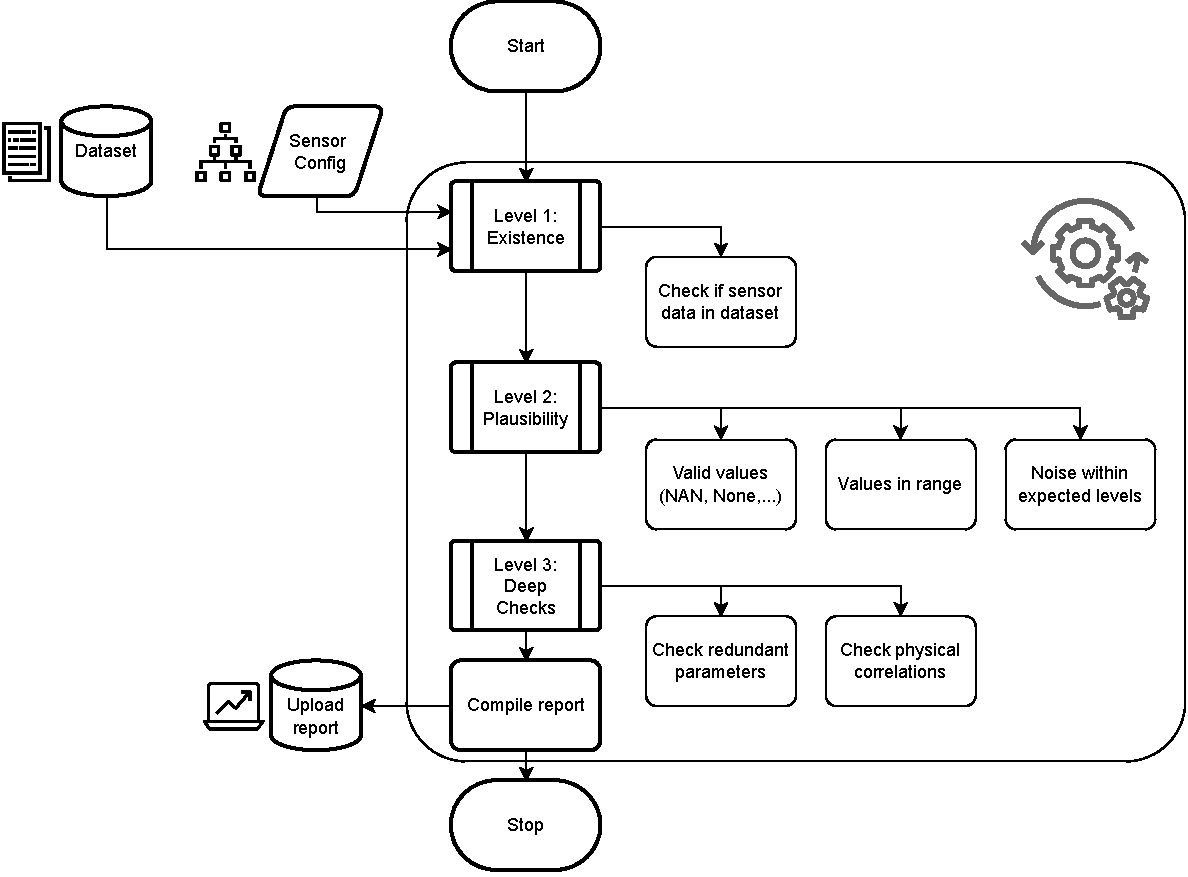
\includegraphics[width=\textwidth]{SHM_simplified}
    \caption[The general, proposed SHM Architecture]{The data flow architecture proposed within this work. Starting with the configuration and dataset as fundamental process inputs feeding the data-processing, algorithmic step. Within the algorithmic step three distinct functions are proposed checking for existence of sensors in the dataset followed by the Plausibility step which checks sensor singularly without other sensors as context and finally the step of Deep Checks in which a correlation check is performed with a custom algorithm. The results from the three steps are then compiled into a data quality report which then can be visualized.}
    \label{fig:SHM_simplified}
\end{figure}

\subsection{Introduction to FMEA}

Motivated by the desire to warn operators of system failure the FMEA has a relatively simple goal. To detect failures and faults and alert the user to avoid further damage, costs and downtime. This naturally establishes it as one of the pillars of automation. \cite{isermann_fault-diagnosis_2006} Since automated systems are only as smart as their creator, methods have to be put into place assuring their high level of quality, guaranteeing smooth operation which in turn spawns and motivates the entire field of FMEA. In recent years, especially systems based on machine learning (ML) approaches have come into play due to widely available cheap computing power as well as increasingly optimized training algorithms. Due to the scope of this work this ML-approach however remains to be addressed at a later point.


In the following, state of the art non ML approaches are introduced preceded by a brief theoretic section on statistics for completeness. The FMEA methods then outlined feature the principal component analysis (PCA) used in live monitoring \cite{xiao_diagnostic_2006}, Pseudo Transfer Functions (PTFs) in control theory \cite{aljanaideh_aircraft_2015}, parity equations as well as grey box models using parameter tuning. \cite{isermann_fault-diagnosis_2006} In addition, some methods from the GNSS field are presented since much of GNSS research is public in contrast to most control algorithms for aircraft systems.

\paragraph{Statistical methods}
%todo: dickes todo bei der statistik. FUCK!
In the following, fundamental statistical methods are shown to prepare the fundamentals for the proceeding SHM steps in Level 1, 2 and 3. Since the focus of this work lies in signal analysis, relevant methods from \textcite{smith_scientist_1999} are proposed.
%TODO: bilder beschreiben
\begin{figure}[h]
    \centering
    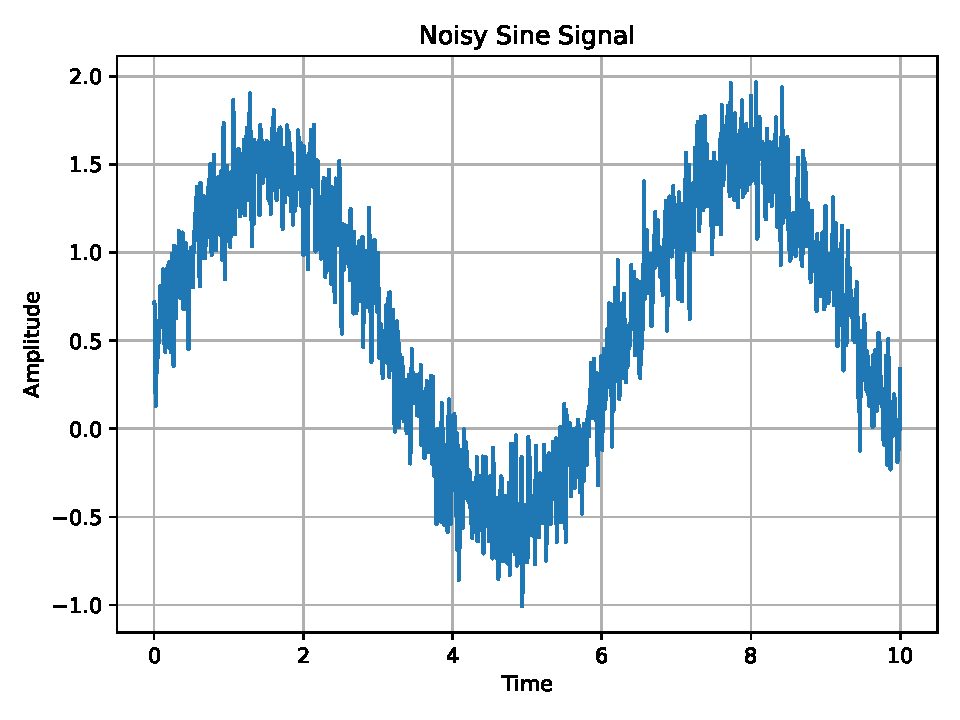
\includegraphics[width=.7\textwidth]{python_functions/images/statistic_functions_clean}
    \caption[Noisy Sine Signal]{A sample sine signal with some white noise to illustrate the following statistical methods.}
    \label{fig:statistics_clean}
\end{figure}

Signal properties are examined for a given signal in Figure \ref{fig:statistics_clean}

%Sensors generally produce errors within expected forms of output. -Noise -Measure using Covariance --> autocovariance -Offset -No response

%tatistical representation of: Mean

\cite[S.13-17]{smith_scientist_1999}

Time continuous mean
\begin{equation}
    \label{eq:mean_cont}
    \mu=\frac{1}{T} \cdot \int_T x(t) d t
\end{equation}
Time discrete mean:
\begin{equation}
    \label{eq:mean_disc}
    \mu=\frac{1}{N} \cdot \sum_{i=1}^{N} x_i
\end{equation}




The variance $\sigma^2$ is a metric for the signal's behavior. It expresses the mean squared deviation from the mean.

Time
\begin{equation}
    \label{eq:var_cont}
    \sigma^2=\frac{1}{T} \cdot \int_T[x(t)-\mu]^2 d t\\
\end{equation}

\begin{equation}
    \label{eq:var_disc}
    \sigma^2=\frac{1}{N} \cdot \sum_{i=0}^{N}\left[x_i-\mu\right]^2
\end{equation}

The standard deviation is derived from the variance. Its value gets square-rooted to better represent the power (magnitude of the amplitude).

Standard Deviation
\begin{equation}
    \label{eq:stdev_disc}
    \sigma = \sqrt{\sigma^2}
\end{equation}

\begin{figure}[h]
    \centering
    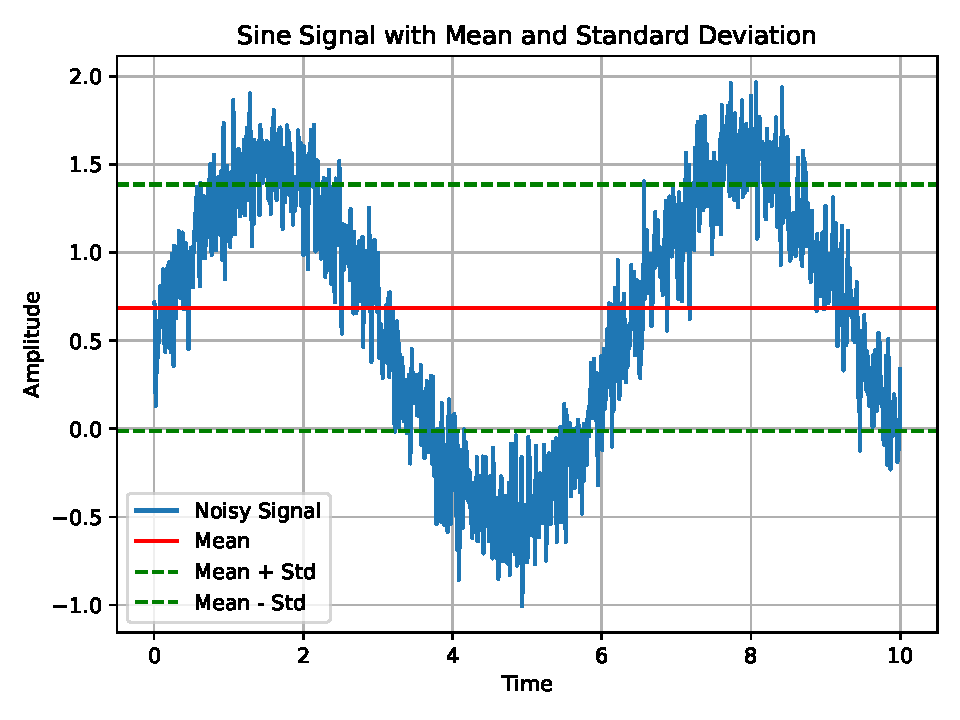
\includegraphics[width=.7\textwidth]{python_functions/images/statistic_functions_basic}
    \caption[Signal analysis with $\mu$ and $\sigma$]{Signal with $\mu$ and $\sigma$ borders for upper and lower limit}
    \label{fig:statistics_basic}
\end{figure}

Mean and the standard deviation don't represent the desired metrics in some use cases. Rather more important is a comparison between the two. Hence, the Signal-to-Noise ratio (SNR) is used to compare and condense the mean and standard deviation by dividing the mean by the standard deviation.

\begin{equation}
    \label{eq:snr}
    SNR=\frac{\mu}{\sigma}
\end{equation}
Another parameter is the coefficient of variation (CV) which is the standard deviation divided by the mean and multiplied by 100\%. Effectively displaying the inverse of the SNR.

\begin{equation}
    \label{eq:coeff_var}
    CV = \frac{\sigma}{\mu}100\%
\end{equation}

\begin{figure}[h]
    \centering
    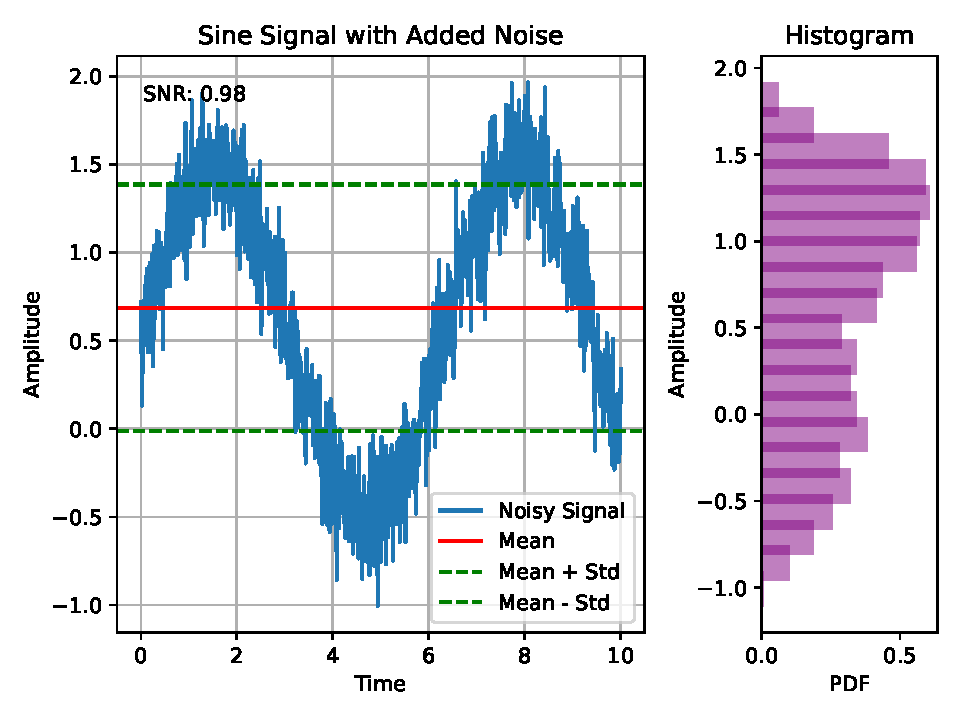
\includegraphics[width=.7\textwidth]{python_functions/images/statistic_functions_full}
    \caption[Full Signal Analysis]{The Sine Signal with $\mu$, $\sigma$, SNR and a Histogram giving more in-depth information on the signal 's behavior.}
    \label{fig:statistics_full}
\end{figure}

An arising problem based on the SNR and CV are however that they scale based on the mean value. Should the mean value lie at about 0 for e.g. a sensor of an aircraft control surface, the signal to noise ratio will be relatively high compared to an acceleration sensor in z axis with a constant offset of 1g. Practical example for mean and standard deviation in a given signal are overlaid in Figure \ref{fig:statistics_basic}
To evaluate a signal according to the quantities the next logical step is the probability mass function (PMF) \ref{eq:pmf}. This part of signal evaluation is shown in the following Figure \ref{fig:statistics_full} by adding a histogram to the analysis which counts the signal points lying within discretized value ranges.

\begin{equation}
    f(x)=\frac{1}{\sqrt{2 \pi \sigma^2}} e^{-\frac{(x-\mu)^2}{2 \sigma^2}}
    \label{eq:pmf}
\end{equation}

Building upon these factors the covariance is introduced as a measure for comparing signals to each other. First the signal gets translated to have a mean value of 0 and then all values of the first series at a certain point $t$ are multiplied with the points of the second series as displayed in the time continuous covariance function.
$$
cov(t, x)=\frac{1}{T} \cdot \int_T[x(t)-\mu] \cdot[x(t-\tau)-\mu] d t
$$
For the time-discrete covariance function follows henceforth:
$$
cov(k, x)=\frac{1}{N} \cdot \sum_N\left[x_i-\mu\right] \cdot\left[x_{i-k}-\mu\right]
$$
Based upon this the autocovariance for a series which compares a series' signal to itself can be represented as:
$$autocov(x) = cov(x,x)$$

Going further, the Pearson coefficient within a correlation matrix is reached by scaling the covariance matrix by the standard deviation: \cite{smith_scientist_1999}

$$\rho_{x,y} = corr(x,y)=\frac{cov(x,y)}{\sigma_x \sigma_y}$$

With the limits of correlation being -1 for total inversely proportional correlation and 1 for total correlation. A total independence for $\rho_{x,y}=0$ is not given since Pearson coefficient only detects linear correlations and not nonlinear behavior. Other correlation methods as rank-correlation (Spearman, Kendall) that detect change correlations are possible but are more complex in the implementation.
%TODO: motivate check levels here. Tell story why it is important

\subsubsection{Summary and Motivation}

Based upon this groundwork, methods for the three levels of the SHM are proposed. State of the Art solutions are discussed for each Level based on the common statistical methods proposed in the previous section.

\subsection{Check 1: Existence}
In the first Level of the SHM it is checked whether parameter data exists in the database. This is checked by comparing the DAQ-configuration to the actually measured data. Within step two, single sensor signals are examined by themselves, saving resources by iteratively working on each sensor. This approach also allows easy parallelization of tasks due to the encapsulation of each task. Step three allows the integration and correlation of different sensor signals. Allowing more complex FMEA systems.

Within the first step, the main challenge lies within the acquisition of sound configuration data. Errors may occur as early as the configuration step due to human error. Making it the first level of defense against simple mistakes.

\subsection{Check 2: Plausibility}
\label{chap:2-plausibility}

Within the plausibility check the single parameter is checked against limits that shall be preconfigured for each parameter. Various methods are examined. The primary focus is checking the value against limits to detect extreme values that are unrealistic. Within the next step, the series is transformed with the noise or other desired attributes being extracted. These attributes can then in turn be checked against other limits. For the noise, various known methods are examined to create a heuristic for noise approximation. Of course, noise approximation models range in complexity and detail from a simple moving window approximation into Fourier transforms (Fast-Fourier-Transform (FFT), Short-Time-Fourier-Transform(STFT), Wavelet Transform (WT) and into advanced works such as language-processing models \cite{hendriks_noise_2008} which exceed the scope of this work and may be implemented at a later date.

These functions are evaluated into a ranking and displayed in Table \ref{tab:lvl2_comparison}. After brief evaluation, the Short-Time-Fourier Transform is considered due to its comparability among sensor signals. Allowing to compare movement activity by amplitude.
\begin{table}[h]
    \centering
    \caption{Comparison of Level 2 Noise approximation algorithms (empty circle - low rating)}
    \begin{tabular}{@{}lllll@{}}
        \toprule
        Noise algorithm:      & Moving Average & FFT       & STFT      & WT        \\ \midrule
        Implementation Effort & \pie{90}       & \pie{270} & \pie{180} & \pie{360} \\
        Result Quality        & \pie{90}       & \pie{180} & \pie{270} & \pie{360} \\
        Real-Time Performance & \pie{360}      & \pie{180} & \pie{270} & \pie{90}  \\ \bottomrule
    \end{tabular}
    \label{tab:lvl2_comparison}
\end{table}
%todo: backlog todo: graph comparing results of lvl2 functions. check position
The STFT algorithm is then implemented preliminary by using a short time window of 256 samples and then collapsing the resulting spectrogram by time. This results in an averaged amplitude value for each timestep that is detrended. Leading to a scalar value, upon which the noise of each value can be mapped.

\subsection{Check 3: Parameter Correlation}
Physically correlating and involving parameters into the anomaly detection of other parameters is the next logical step. It is primarily considered to use conventional non ML-approach using known correlations of parameters and perhaps allowing some grey box approaches for fine-tune limits and finding unknown correlation. A primary desire is to generate a model that is not hardcoded but easily expandable to satisfy various data-generators. A few non-ML FMEA approaches are presented in the following paragraphs to build a primary overview over the wide field of FMEA.

\subsubsection{Principal Component Analysis}

The Principal Component Analysis (PCA) was first introduced by Karl Pearson in 1901 (\cite{pearson_liii_1901}) and has since become a popular method to analyze datasets and detect correlations. The PCA works by reducing the dataset dimensions using covariance of parameters relative to each other. This results in a method that needs minimal user input but delivers a condensed data overview. The only input needed is the number of dimensions into which data shall be condensed into, the so called Principal Components (PCs).

The functionality, applications as well as usability within the context of this work are discussed below.

\begin{description}
    \item[Functionality]\hfill

    The PCA is a method that allows to reduce the information parameters of a dataset into a few principal components or dimensions. Generally, this is specified as the operation of multiplying the original dataset $X_{Nxm}$ with the timesteps $N$ and the measurement parameters $m$ with the Permutation Matrix $P_{mxr}$. This results in the transformed principal components (PC) $T_{Nxr}$ with $r$ being number of reduced dimensions or also the number of Principal Components. This transformation is defined as:

    $$T_{Nxr} = X_{Nxm}  P_{mxr}$$

    P being the permutation matrix that transform the original data into the principal components. The overall strategy to generate a PC is shown in Figure \ref{fig:pca_variance} as finding a function between two parameters $x_1$ and $x_2$ that maximizes the variance of data in a newly generated principal component. However, drawbacks arise using this approach since the variance optimization only happens linearly and is not able to function for nonlinear correlations similar to a standard Pearson-Coefficient Correlation matrix. \cite{handl_multivariate_2017}

    \begin{figure}[h]
        \centering
        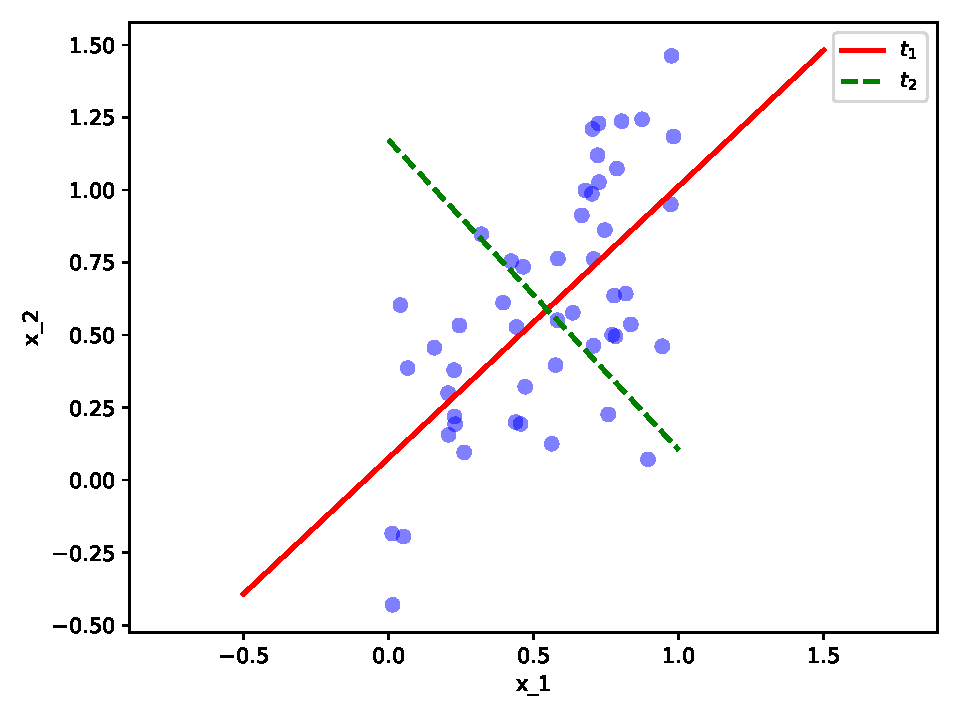
\includegraphics[width=0.5\textwidth]{python_functions/images/pca_variance}
        \caption[Illustration of a singular PCA Transformation]{Parameters $x_1$ and $x_2$ get converted into principal components $t_1$ and $t_2$ by optimizing for minimal variance of blue dots along the red line.}
        \label{fig:pca_variance}
    \end{figure}

%%principal component
    PCs can be created in any direction. Where input is needed however is the number of Principal components that shall be kept. A cutoff value can be defaulted to but this may not be feasible for multidimensional systems such as the flight test data that is at hand.


    Eliminating a principal component becomes easy if parameters show a direct correlation such as in Figure \ref{fig:pca_variance}. The gatherings of $t_2$ then mostly consist of noise and can be safely discarded.

    \item[Utilization]\hfill

    \begin{figure}[h]
        \vspace{-20pt}
        \centering
        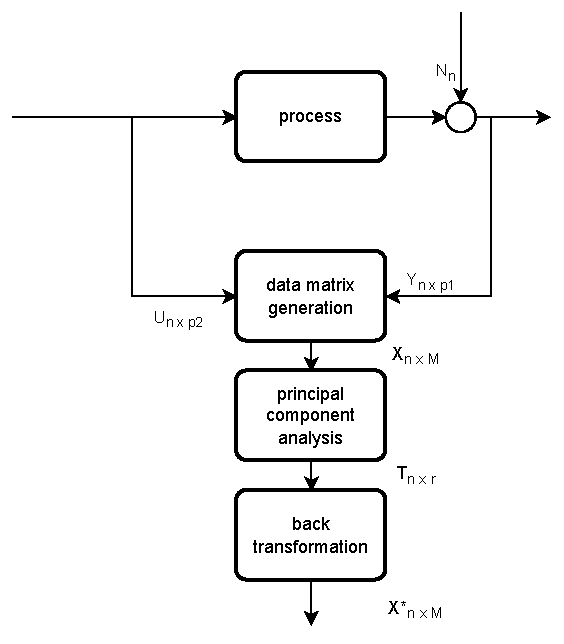
\includegraphics[width=0.48\textwidth]{pca_FD}
        \caption[PCA for residual generation in FMEA]{Process input U and Sensor Measurement Y get transformed into state X and fed into a PCA. N indexes timesteps and $X^*$ is the predicted output.\cite[p.268]{isermann_fault-diagnosis_2006}}
        \label{fig:pca_FD}
    \end{figure}

    This analysis method is especially helpful for datasets for which correlations are unknown such as biomedicine in which marker correlation needs to be identified. But even for aerospace contexts it may prove helpful for large quantities of data in which correlations are unknown e.g. for parameter identification as well as perhaps aeroelastic applications in which vast amounts of acceleration sensors and strain gauges are present and used to explain dynamic behavior of the aicraft's structure.

    In these applications the PCA is a great tool to get a first overview over the data. For more refined analysis however, it lacks detail since it generally uses linear optimization as and may be prone to overfitting for redundant input parameters. In these cases, it may be sensible to use optimized PCA approaches or an entirely different analysis system such as ML-approaches.

    The PCA can be defined as a condensation of a dataset into fewer parameters. These are then defined as principal components. These principal components can also be transformed back into the original parameters making the entire process reversible and allowing to create a data model. Based upon this model it is possible to then calculate residuals in order to possibly quantify the error. E.g. \textcite{isermann_fault-diagnosis_2006} presents a process for an autotuning PCA FMEA that can be used for real-time Fault Detection applications.

    \item[Assessment]\hfill

%%motivation

    The principal component analysis is based on correlation principles and allows reduction of datasets into independent components. Applications in an aerospace context include detection of previously unknown correlations between parameters and complex interactions in aeroelastics or otherwise large datasets. Usage however is associated with a certain effort since information needs to be preprocessed to a certain degree, reducing dimensions previous to processing in order to avoid feeding in redundant parameters.

%%variance

%Generally, we want to transform the Matrix X into the transformed Matrix T containing all Principal components with the count $r<m$. To perform this operation we introduce the Permutation Matrix P leading to:
%$$T_{Nxr} = X_{Nxm}  P_{mxr}$$
%A principal component gets created by condensing two parameters in the direction of most variance to each other. This is a classical optimization problem


%%pca general analysis (plots)
%%pca uses in fault detection

\end{description}

\subsubsection{Pseudo Transfer Functions}


Novel developments in control theory port methods from previous applications in Structural Health Monitoring (StHM) whose original purpose is to analyze building and structure oscillative behavior such as frequency and amplitude to detect critical values. These StHM methods use multiple sensor data to detect anomalies in single sensors. In novel research these methods which were in the frequency domain have been transferred into the time domain, making them usable for general time series analysis. This process uses the Transmissibility function $\mathcal{T}$ using dynamically generated Markov-parameters for which a Pseudo Transfer Function (PTF) then needs to be found. Essentially spanning up a matrix of markov parameters similar to a correlation matrix. These Markov parameters then get tuned within the beginning of the measuring period after which a conistent model allowing to generate a residual to detect errors. \cite{khalil_transmissibility-based_2022, khalil_transmissibility-based_2022-1, wolter_anwendung_2014}

\begin{description}

    \item[Functionality]\hfill

    Following the recipe for a modeled aircraft based on sensor data $y$ the parameters $x$ and $u$ of the aircraft are attempted to be simulated. \textcite{aljanaideh_aircraft_2015} shows that this approach works for linking the angular velocities for the aircraft axes $\omega_x$, $\omega_y$, $\delta_{drift}$(drift angle) with $\omega_z$. The examined approaches include the transmissibility function $\mathcal{T}$ that models the system output without having to take the unknown system input into consideration.


    \item[Utilization]\hfill

    Since this is a relatively new development with no broad implementations yet existing. It is to note however, that the origin of this method in StHM might possess more implementations. Within multiple publications by the author this process is applied for various purposes such as the Aircraft Sensor Health Monitoring \cite{aljanaideh_aircraft_2015} and a newer addition including SHM for a Platoon of autonomous robots \cite{khalil_transmissibility-based_2022}.

    \item[Assessment]\hfill

    This approach seems especially suitable for real-time implementations and may also be used in postprocessing. It comes however with the penalty of not being usable straight out of the box since no python implementations exist so far. For future work, this may be implemented to evaluate its capability against other algorithms. It also remains to be seen how well this algorithm performs on large datasets and how much preprocessing effort needs to be undertaken.
\end{description}

\subsubsection{Parity Equations}
\label{chap:parity_equation}
Parity Equations work by modelling the physical state of a system in normal working conditions. They are based on known physical relationships between sensor measurements and generate a residual. This residual is then continuously checked during operations and once it reaches or exceeds a previously defined threshold it notifies the system's operator. \cite{isermann_fault-diagnosis_2011}

\begin{description}
    \item[Functionality]\hfill

    The Parity workflow separates into the two steps of calculating the physical state and generating a residual and then interpreting the residual.

    \item[Utilization]\hfill

    Parity Equations are employed in systems in which the physical correlations are well-known. They allow fusion of various parameters into system state variables to then generate residuals for single parameters to determine the parameter errors.

    \item[Assessment]\hfill

    Since the relations of the aircraft systems and behavior have historically been subject of extensive research the Parity equations lend themselves to be considered within this context. Extensive tuning is however integral part of Parity Equations since physical correlations as well as residual thresholds need to be tuned to avoid amassing false positives.
\end{description}

\subsubsection{Grey Box models}

Another method for system modelling lies in grey box models. The "grey" attribute arises from the property that these systems have baseline constraints that may be set and some degrees of freedom such as tuning parameters. These tuning parameters are then tuned against a set of previously defined training cases to satisfy the constraints. This represents an approach that works with limited system knowledge and implementations such as the PTF are implementations of this model. \cite{isermann_fault-diagnosis_2006}

%\paragraph{Functionality}

%\paragraph{Utilization}

%\subsubsection{Assessment}
%Far more

%model based fault detection(isermann)
%-parameter estimation (process modeling with linear or nonlinear functions, unknown process parameters are modeled by residual minimization)
%-parity equations ()
%-state estimation (kalman), state/output observers (for known process parameters, )


%\paragraph{RAIMS}
%Examination of Receiver autonomous integrity monitoring (RAIM) from GNSS applications.
%basic principle 1 in 1 out basic
%2 in 1 out mean solution. Detect discrepancies 1. simple solution: take average 2. detect discrepancies but still take average
%3+ in 1 out. 1. take average 2. detect value with strong variations and isolate (it is assumed that only 1 sensor is faulty)
%2.1 predict value and deny value if it is larger than 3 times standard deviation (Wen07, 239).
%implementation details. see [Bro92]

\subsubsection{FMEA Evaluation}

An algorithm for evaluating data quality in Level 3 must now be found based on these state of the art approaches. \textcite{zhang_bibliographical_2008} presents a general overview over the field of FMEA which allows to be split into the two main categories of model and data-based methods which are dependent on the system knowledge that shall be introduced into the FMEA. Both then carry two fields within of quantitative and qualitative methods which get applied for conditional modeling and less stringent data types.
\begin{figure}[h]
    \centering
    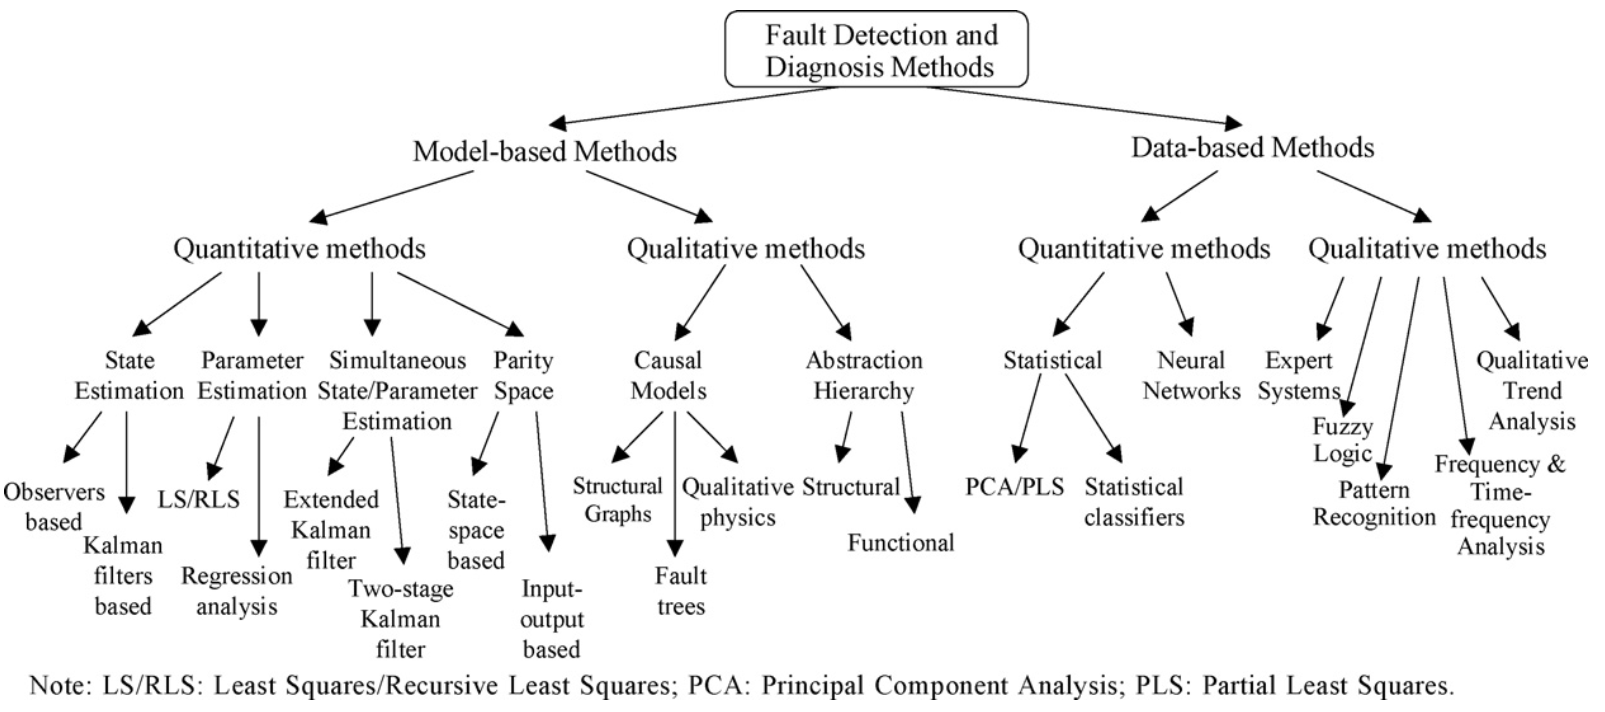
\includegraphics[width=1\textwidth]{FMEA_methods}
    \caption[A grand FMEA overview \cite{zhang_bibliographical_2008}]{An overview over various kinds of FMEA satisfying a broad range of specific requirements that may be posed as system specifications. \cite{zhang_bibliographical_2008} While clear distinctions must be made between quantitative and qualitative methods the main distinction lies in the amount of system knowledge provided to the method.}
    \label{fig:FMEA-methods}
\end{figure}
Within this endeavor it however needs to be considered that this summary of FMEA methods barely scratches the surface. Far more FMEA variations exist than shown in Figure \ref{fig:FMEA-methods} and the effort within this work is limited. The goal is then to develop a primary heuristic that can deliver results whose primary purpose is to actually exist and not still be stuck in development. Additional important factors also are the FMEA-method's actual performance. Possible issues arise while comparing reliability. Especially in aerospace with multiple independent axes a false correlation may be detected due to circumstances. E.g. for a flight performing multiple consecutive landings it is possible for the Distance Measuring Equipment (DME) measuring distance to the airport to correlate with altitude and speed since all decrease and increase simultaneously. Simultaneously, employing no/low knowledge models enables rapid results eliminating the need for any degree of system knowledge.


\begin{table}[h]
    \centering
    \caption{Comparing FMEA solutions by their respective usability}
    \begin{tabular}{@{}llll@{}}
        \toprule
        Noise algorithm:             & Implementation Effort & System Knowledge & Reliability \\ \midrule
        Principal Component Analysis & \pie{270}             & \pie{0}          & \pie{180}   \\
        Pseudo Transfer Functions    & \pie{360}             & \pie{180}        & \pie{270}   \\
        Grey Box Models              & \pie{270}             & \pie{180}        & \pie{180}   \\
        Parity Equations             & \pie{90}              & \pie{360}        & \pie{360}   \\ \bottomrule
    \end{tabular}
    \label{tab:lvl3_fmea_comparison}
\end{table}

In Table \ref{tab:lvl3_fmea_comparison} the introduced FMEA-schemas are evaluated on their viability to use within this work. While PTF as well as other Grey-Box models exist, they need considerable effort within their primary implementation and then their respective training. Since the research and development of a novel, optimal FMEA is also not focal point of this work since it is rather more important to generate a holistic heuristic, solving first and foremost the basic problems associated with basic errors. Hence, Parity equations are chosen to be developed further within this work. Generating a dynamic model of the aircraft physical correlations that allows itself to be expanded for future use. It remains to be seen now, how well this work's architecture for integrating these FMEA may hold up in regard of testing these methods in future work.


% state space:matrix impl. linear, very powerful+scalable,
% Simulink: nonlinear, very powerful, license cost, not dynamically configurable -->manual interaction
% FMEA python solutions: higher effort in implementation, dynamically automatable
% -->python implementation with dynamically modifiable configuration

\subsection{Context within Aerospace Applications}
The previously mentioned subset that will be examined within this work is the altitude of the aircraft. In the ISTAR the altitude can be determined by using the barometric altitude and the altitude determined by the Global Navigation Satellite System (GNSS). To implement a Parity Equation the system knowledge needed to create these models is introduced. In the following the exemplary implementation of a barometric system is presented followed by considerations needing to be made when examining the GNSS system and comparing it to the barometric system.

\subsubsection{Barometric Altitude}
For the Parity model, the barometric altitude is introduced to compare experimental pressure sensors with the aircraft's barometric altitude.

The International Standard Atmosphere (ISA) is the conventional method of measuring an aircraft's altitude based on air pressure and the industry standard. \cite{iso_standard_1975} The method can be understood as a function of pressure and reference pressure (differing based on weather) which results in an altitude. The assumptions for each layer of the atmosphere are shown in table \ref{tab:isa_temp}.

\begin{table}[h]
    \centering
    \caption[International Standard Atmosphere Layers\cite{zhang_bibliographical_2008}]{Atmospheric Layers as defined in the International Standard Atmosphere \cite{iso_standard_1975}}

    \begin{tabular}{@{}cccc@{}}
        \toprule
        Atmospheric  & Geopotential      & Temperature T     & Temperature           \\
        Layer        & Altitude {[}km{]} & at bottom {[}K{]} & gradient a {[}K/km{]} \\ \midrule
        Troposphere  & -2-0              & 301.15            & -6.5                  \\
        Troposphere  & 0-11              & 288.15            & -6.5                  \\
        Tropopause   & 11-20             & 216.65            & 0                     \\
        Stratosphere & 20-32             & 216.65            & 1                     \\
        Stratosphere & 32-47             & 228.65            & 2.8                   \\
        Stratopause  & 47-51             & 270.65            & 0                     \\
        Mesosphere   & 51-71             & 270.65            & -2.8                  \\
        Mesosphere   & 71-80             & 214.65            & -2                    \\ \bottomrule
    \end{tabular}
    \label{tab:isa_temp}
\end{table}

Based on these constants the general equation for pressure within an atmospheric layer with a nonzero temperature gradient is shown in equation \ref{eq:baro_Tvar}. \cite{iso_standard_1975}

\begin{equation}
    \frac{p}{p_0}=\left(1+\frac{a \cdot\left(h-h_0\right)}{T\left(h_0\right)}\right)^{\frac{-g}{a \cdot R}}
    \label{eq:baro_Tvar}
\end{equation}

\begin{conditions}
    p      & pressure at current altitude [Pa]                              \\
    p_{0}  & reference pressure [Pa]                                        \\
    h      & current altitude   [m]                                            \\
    h_{0}  & reference altitude [m]                                         \\
    T(h_0) & temperature at reference altitude [K]                          \\
    a      & ISA Temperature gradient (see table \ref{tab:isa_temp}) [K/km] \\
    g      & gravity constant $(9.80665) [m/s^2]$                           \\
    R      & Ideal Gas Constant  $(287.05287)[m^2/( K\cdot s^2)]$
\end{conditions}

Transforming this formula for altitude resolves into equation \ref{eq:h_baro_Tvar}

%\[1 + \frac{a}{T(h_0)}\cdot (h-h_0) = \left(\frac{p}{p_0}\right)^{\frac{1}{\frac{-g}{a \cdot R}}}\]
\begin{equation}
    \rightarrow h = \left(\frac{p}{p_0}^{\frac{-a \cdot R}{g}}-1\right)\frac{T(h_0)}{a}+h_0
    \label{eq:h_baro_Tvar}
\end{equation}

\paragraph{Constant layer temperature}

Since equation \ref{eq:baro_Tvar} does not represent the conditions for a constant temperature with $a = 0$ the original equation needs to adapted and it follows from \textcite{iso_standard_1975}:

\begin{equation}
    \frac{p}{p_0}= \exp\left(\frac{-g}{R \cdot T(h_0)}\cdot(h-h_o)\right)
    \label{eq:baro_Tconst}
\end{equation}


The following equation \ref{eq:h_baro_Tconst} then resolves for the altitude based on pressure ratio within a layer with constant temperature.


%$$ln(\frac{p}{p_0}) =\frac{-g}{RT(h_0)}\cdot(h-h_o) $$
\begin{equation}
    h = ln(\frac{p}{p_0})\cdot \frac{R \cdot T(h_0)}{-g}+h_0
    \label{eq:h_baro_Tconst}
\end{equation}

\paragraph{Logic Flow}

The process to then actually calculate a barometric altitude is displayed in Figure \ref{flow:ISA}. The input is p and $p_0$ with p being the measured pressure via the aircraft's static ports and $p_0$ being the reference pressure that is manually set by the pilot with the standard pressure being $p_{std} = 1013.25$hPa which varies depending to the weather.


\begin{figure}[h]
    \centering
    \begin{tikzpicture}[
        node distance=3cm,
        terminal/.style={draw, rounded rectangle,rounded corners=10pt, text centered, minimum height=4em, minimum width=6em},
        io/.style={draw, trapezium, trapezium left angle=70, trapezium right angle=110, minimum height=2em, minimum width=4em},
        process/.style={draw, rectangle, text centered, minimum height=2em, minimum width=5em},
        decision/.style={draw, diamond, aspect=2, text centered, minimum height=2em, minimum width=3em}
    ]
% Nodes
        \node (start) [draw, terminal] {Start};
        \node (input) [draw, io, above of=start] {$p, p_{0}$};
        \node (data) [draw, io, below of=start] {ISA};
        \node (getlayer) [draw, process, right of=start, align=center] {[1]\\get layer\\from table \ref{tab:isa_temp}};
        \node (decide) [draw, decision, right of=getlayer, align=center] {[2] is a=0?};
        \node (a) [draw, process, below right of=decide, align=center] {[3.2]   $a=0$\\Get p with eq. \ref{eq:h_baro_Tconst}};
        \node (notA) [draw, process, above right of=decide, align=center] {[3.1]  $a \neq 0$\\Get p with eq. \ref{eq:h_baro_Tvar}};
        \node (output) [draw, io, below right of=notA, align=center] {[4]\\ altitude output};
        \node (stop) [draw, terminal, right of=output] {Stop};

% Arrows
        \draw [->] (start) -- (getlayer);
        \draw [->] (input) -| (getlayer);
        \draw [->] (data) -| (getlayer);
        \draw [->] (getlayer) -- (decide);
        \draw [->] (decide) |- node[anchor=east]{Yes} (a);
        \draw [->] (decide) |- node[anchor=east]{No} (notA);
        \draw [->] (a) -| (output);
        \draw [->] (notA) -| (output);
        \draw [->] (output) -- (stop);
    \end{tikzpicture}

    \caption{An algorithm to determine barometric altitude $h$ based on $p$ and $p_0$}
    \label{flow:ISA}
\end{figure}



In step 1 the current atmospheric layer gets found by matching the MSL-pressure ratio  $\frac{p}{p_0}$ to precalculated boundary values of layers based on table \ref{tab:isa_temp}. After determining the layer and the value for temperature coefficient $a$, the altitude can quickly be determined by inserting layer properties as well as the pressure ratio into their respective altitude equation (step 3.1 and 3.2 in flowchart \ref{flow:ISA}). In the final step 4 the altitude is returned.

\subsubsection{GNSS}
In addition to the barometric altitude, the position of the ISTAR is also determined by the Global Navigation Satellite System (GNSS) in the aircraft. For reference, the aircraft altitude generally is defined as the displacement of the aircraft from Mean Sea Level (MSL). It is important to note that the earth can generally be described as an ellipsoid due to its rotational shape in a geodetic context resulting in a very close approximation of the earth's shape. However, varying density levels of the earth's crust cause the elevation and sea level to deviate from the ellipsoid shape. This results in a lopsided model that is modeled in the WGS84 (\cite{schwarz_wgs_1998}) system. This is also the altitude that the GNSS system measures. And it will be the reference altitude for the following calculations.
% todo: will this actually be the altitude that will be measured. Isnt the barometric altitude the one to be used? Perhaps differentiate into "reference altitude" for the reference model

Possible errors for each are:

\begin{tabular}[h]{ll}
    Geodetic:            & Inconvenient satellite placements,               \\ & deflection of signals in the atmosphere and signal problems \\
    Barometric Altitude: & Meteorological phenomena such as pressure shifts \\ & or also due to inappropriate reference altitude. \\
\end{tabular}

%todo: von christina: errors in human factors: wrong QNH setting
Going into the standardized World Geodetic System (WGS84, \cite{teunissen_springer_2017}) and the GNSS Altitude however exceeds the scope of this work. In the following, the satellite altitude above Mean Sea Level (MSL) is considered as the reference altitude. Fault detection algorithms within GNSS are described as Receiver Autonomous Integrity Monitoring (RAIM) and are tried and tested within GNSS implementations since high accuracy positioning is valuable for various applications, reaching precisions of up to a few centimeters. Explaining the full function of position calculation exceeds this works' scope. To summarize however, GNSS inputs form an overdefined system of equations which needs to be compensated within some algorithm to form one position based on multiple inputs. \cite{teunissen_springer_2017}

\subsubsection{Summary}
%summarize
The fundamentals of potential algorithms to quantify system qualities have been presented in the past section. The statistical fundamentals have been briefly outlined followed by FMEA implementations from statistics in the shape of Principal Component Analysis (PCA) ranging to implementations from control theory. Advanced models such as machine learning models have not been presented but are generally similar to PCA since they also work without system knowledge and also extract features similar to Principal Components. In addition, the context within the ISTAR has been laid out, introducing the barometric altitude and GNSS systems as the systems that will be focused in the implementation of the Parity Equations.

%When talking about Sensor Health Monitoring (SHM) generally one requirement is made which is to detect failures and suspicious behaviors within a system. The failures then need to be quantified to allow writing algorithms to detect them. If one had a sensor value that differed strongly from its expected values a decision needed to be made how much the sensor value differed from the expected value and where the system would receive the information from. This and further considerations are examined in the following chapter to generate a broad overview over the topic of Sensor Health Monitoring and Fault Detection.


%%%scope of this work
The research within the general quality control field is generally very optimized with most of its research on analytical and traditional methods having been developed and implemented in the late 20th century \cite{isermann_fault-diagnosis_2011}. The new arising challenge faced within this work lies primarily in integrating these existing algorithms to allow evaluation of them. In the future such tool boxing approaches may allow quick and easy comparison of new experimental approaches by e.g. running new experimental ML-routines in such a toolbox to then validate them against existing tried and tested FMEA approaches within frameworks such as the ones developed within this work.

In addition to detecting faults it is also necessary for a SHM to display faults to the systems operator. This may happen in the shape of a display interface or a dashboard that generates fault and reliability ratings. Condensing information for operators is also a necessary part of SHM since suspicious occurrences may be frequent and raw information about events is less helpful than already preprocessed data. This is what is now presented in the upcoming sections, first dealing with the structure in which the metadata will be handled and discussing the origin and destination of data in the SHM context.

%Within this chapter various algorithms and methods that may be used to detect faults are presented first and then followed by considerations in the direction of metadata. Standards for metadata as well as new propositions are examined and the Skystash architecture which is used for data hosting as well as analytic tasks is presented.
\newpage


\section{SHM Metadata Structures}

Data handling as well as structuring the data is essential for fulfilling FAIR criteria in terms of the accessibility and reusability. Thus, necessitating a standardized data and metadata format. In the following, the FAIR principles and the motivation of data handling is presented and then its application in form of data format as well as the metadata format are introduced.

%TODO: intro python, json

\subsection{FAIR guiding principles}

Standardized data handling and following of conventions in regard of data structures always directly clashes with the desire to optimize data structures, making them more efficient, dynamic as well as developing them further. Were data structures once used as purely SQL (tabular format) this has now expanded into a wide array of data structures that are tightly knit into the needs and requirements of their application. Starting from tree structures, going into graph-theory and furthering into unstructured paradigms, these approaches represent the tradeoff between standardization and accurate data representation. The following paragraph discusses the use of FAIR principles to satisfy the standardization aspect while also allowing flexibility within the system to represent the underlying physical systems. The full FAIR principles are shown in Figure \ref{fig:FAIR} detailing the single steps associated with each of the four grand principles.\cite{wilkinson_fair_2016}
\begin{figure}[h]
    \centering
    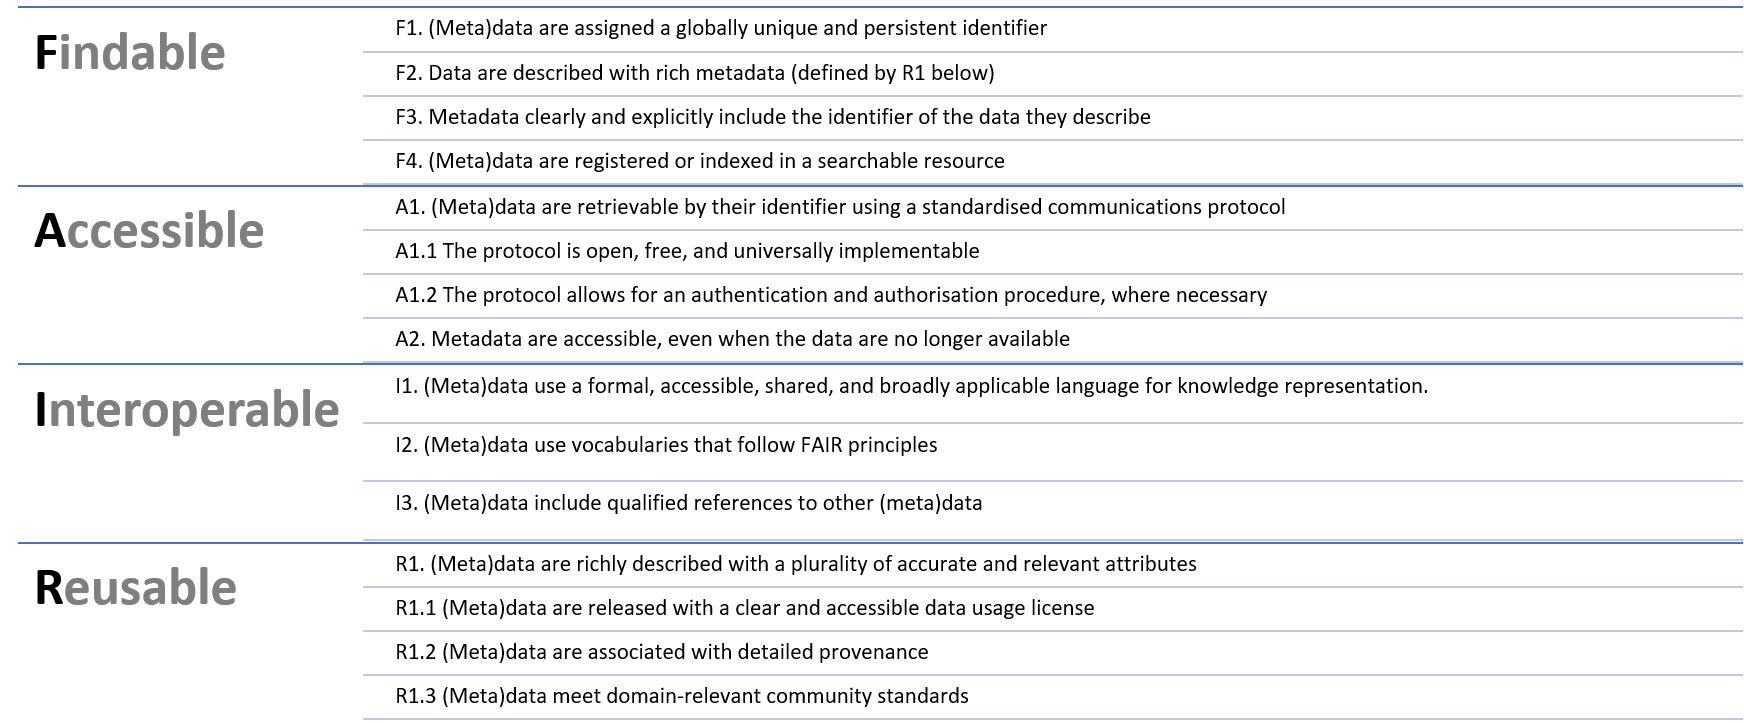
\includegraphics[width=\textwidth]{FAIR}
    \caption[The FAIR principles \cite{wilkinson_fair_2016}]{The full FAIR guiding principles associated with their individual full description. \cite{wilkinson_fair_2016}}
    \label{fig:FAIR}
\end{figure}

\subsubsection{FAIR principles}

Originating from a Dutch alliance of biotechnology institutes in 2015, the FAIR Guiding principles emerged in 2016 as a general best practice guide for research data, referencing best practices

FAIR principles have been published in 2016 by \textcite{wilkinson_fair_2016}. They set the foundation for a standardized and open data culture. Within these principles lie values like open access for data, findable and well tagged datasets, interoperable data by using standardized formats and semantics which guarantee a reusability of data to generate a sustainable process for data usage. Effectively meaning that similar experiments do not have to be performed multiple times when well tagged and formatted data is freely available.


FAIR essentially acknowledges that data analytics have come so far that the data analysis has become very effortless. So effortless however, that a major part of data science consists of formatting and acquiring data. To circumvent this issue in the future and also learn from past data it is then vital to guarantee FAIR principles. This allows to leverage current technology to automate analysis and enable detection of previously undetected correlations within datasets.

\subsubsection{SI-Units}
Units, especially in aerospace contexts, are far from standardized. Most scientific users prefer the International System of Units (SI) due to its ease of use and lack of conversion factors \cite{newell_international_2019}. However, the convention for Pilots and Flight Test Engineers remains imperial within units such as feet, Nautical Miles, knots and so on due to their prominent use in aviation. Naturally SI-units are chosen for the calculations in this work since calculations in SI-units are more efficient as well as less prone to errors. Within this work, the base 1 SI-units will be used (e.g. m, s, N, kg, Pa).

\subsection{Methods}
Within this work it is then necessary to use standardized FAIR frameworks for data and metadata exchange. Since the Skystash, a FAIR research data platform is already in development and in prototypical use within the DLR, the developed algorithm will be tested by working in conjunction with the Skystash. To exchange data, the SOIL (SensOr Interfacing Language) framework will be examined for defining metadata of the aircraft and the FMEA logic itself.

%todo: include ssn ontology as reference. Perhaps use it as reference for graph metadata?
%\cite{dey_organization_2015}

\subsubsection{Skystash}
\label{chap:skystash}
The Skystash is a platform to distribute, analyze and visualize large flight data sets. It is currently in development within the DLR's digital twin project and aims to be a service platform for uploading and sharing the DLR's flight test data. Various requirements are posed from different stakeholders. And large data sets necessitate a platform that can handle these file sizes. Driven by the FAIR guiding principles the Skystash has unique identifiers for each data point and has a powerful search query embedded in its database structure. Such a database also enables data operations since it eases implementation efforts due to the size of data upwards of 2GB per flight, which rapdidly slows down computing on computers with less memory.

%Such as sampling rate. Flight guidance projects may be content with sampling rates as low as 1 Hz. Other stakeholders such as aeroelastic experts may require sampling rates as high as possible and may reach up to 2000Hz within the ISTAR. For this purpose, a dynamic data export is sensible in which users can directly choose sampling rates as well as single parameters from a flight contrary to downloading and working with a whole flight data set averaging up to 2GB of data.

%\section{downloadfunctionalities}
%file sizes too large --> Reduction for on demand parameters and resampling utility Handling of large data sets

%What are Skystash goals to implement, how does it generally work?
The Skystash internal architecture is presented in Figure \ref{fig:skystash_architecture}. A nginx web server builds the centerpiece of the Skystash. It controls web traffic and accepts inputs via a python API as well as the website and redirects it to a keycloak service of the DLR for authentification. After authentification the Stash Service processes the request that has been transferred by nginx and forwards it to the appropriate service and checks it for any errors. The Stash Service is generally the router for three different subsystems. Firstly, a database in a mongoDB format which allows a hierarchical structuring of data and has a native powerful search query, improving Findability of data. Additional python applications can be added to the backend for additional functionality such as upload or import modules for different data formats, allowing straightforward uploads for data. Thirdly, the Service Hub allows for Horizontal Scaling by controlling the docker containers used in the backend which encapsulate each subsystem of the Skystash. If nginx receives a request by the Web GUI it accesses the Web Gui provider to provide the WebUI to the client which itself is written in the Angular Javascript framework. Of great importance is the user management as well which is managed by a keycloak service that accesses the DLR's user management service CoMet.

\begin{figure}[h]
    \centering
    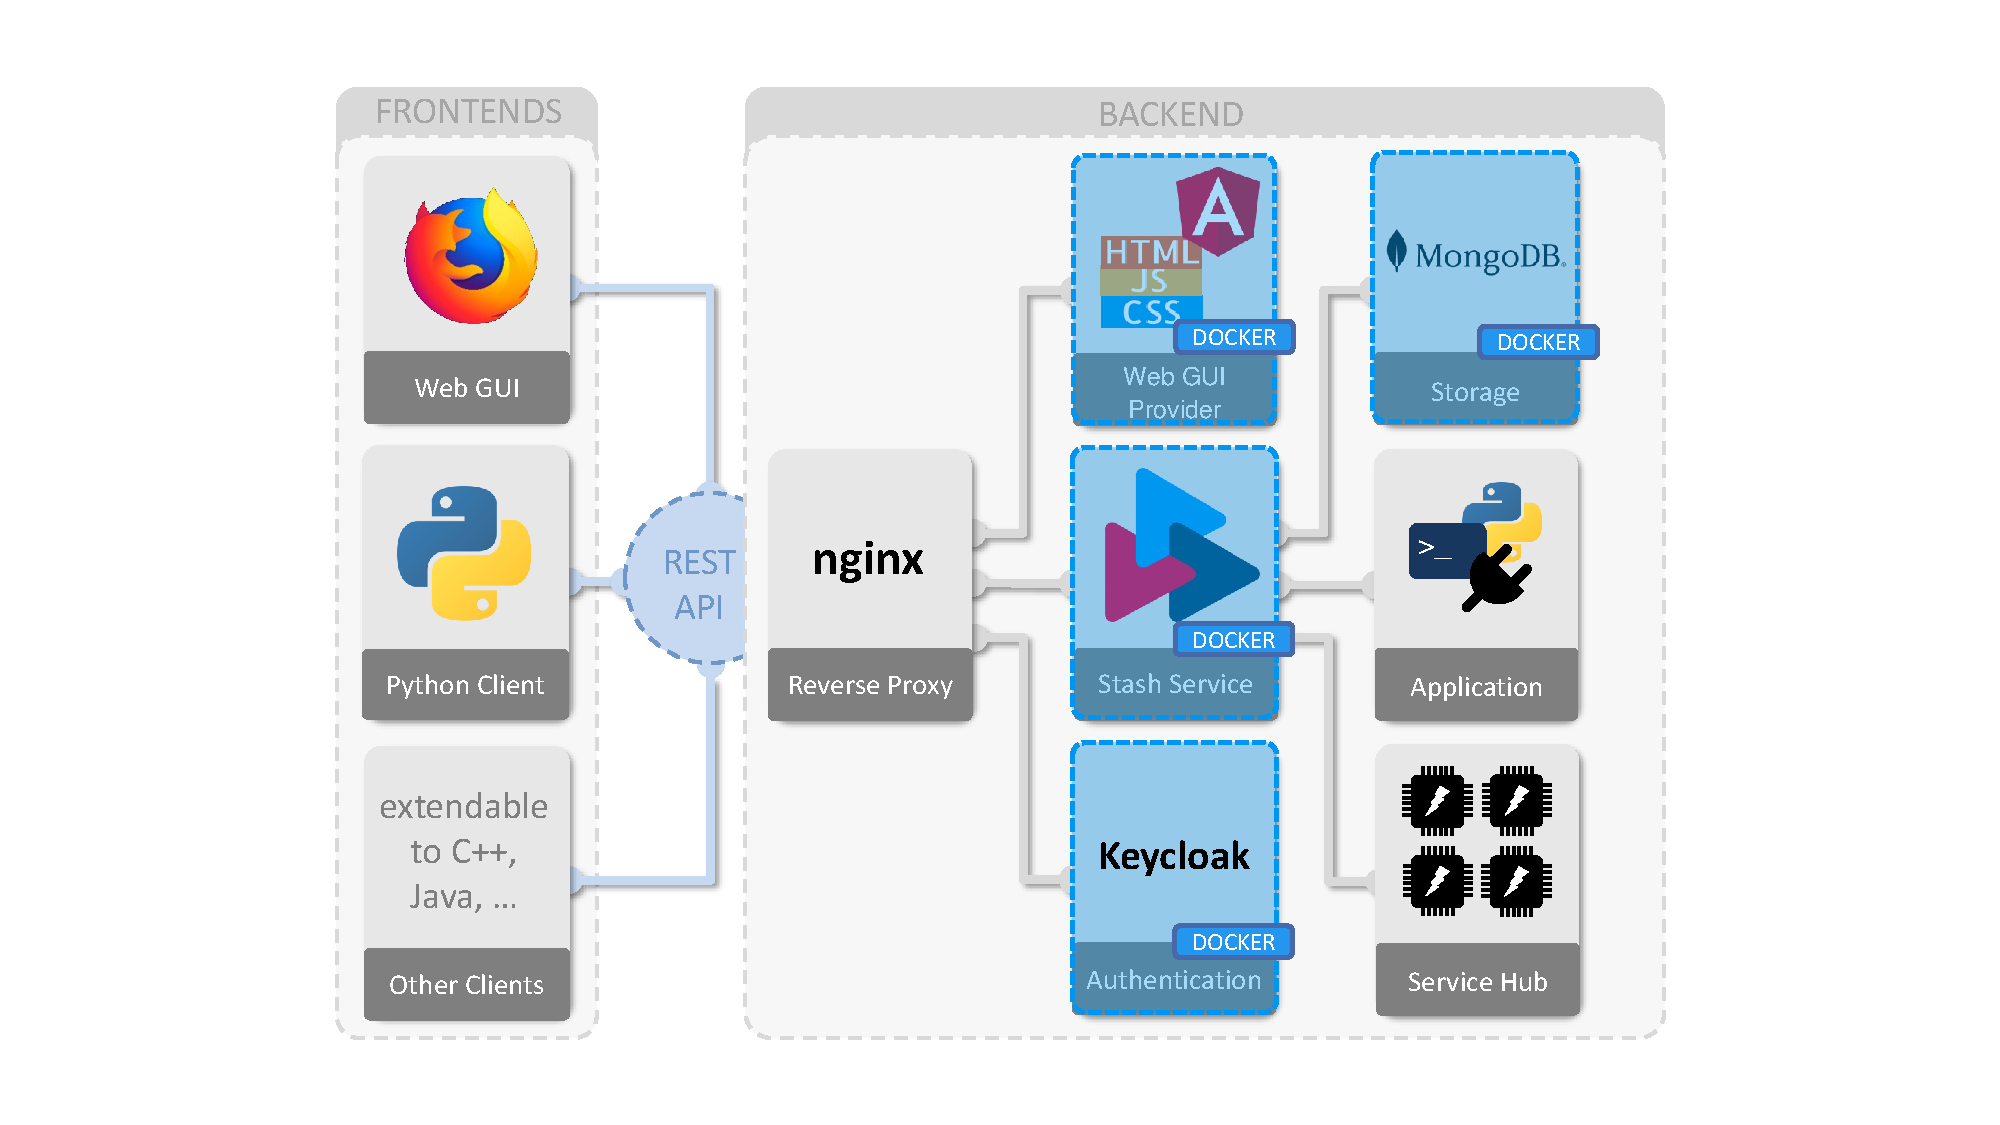
\includegraphics[width=\textwidth]{03_figures/stash_architecture}
    \caption[The Skystash architecture \cite{arts_digital_2022}]{The Skystash architecture signifying the high coupling and low coherency by imlementing a REST API interface in order to spatially separate any interactions with the architecture. The backend of the Skystash uses multiple microservices for different aspects of the software by Routing through the \textit{Stash Service} such as a MongoDB database for storage and python clients for applications. A Service Hub takes care of scaling the infrastructure as a whole. \cite{arts_digital_2022}}
    \label{fig:skystash_architecture}
\end{figure}

Flight test data needs to be perceived within the context of its circumstances to extract all its information. Hence the need for a digital twin arises. Within this context all necessary data shall be compounded to set a central starting point for data exploration and analysis. Figure \ref{fig:digecat_data_sources} shows all data sources that will be gathered. For this works context this means that necessary aircraft configuration data such as location of sensors is available (metadata) next to the actual generated data from the aircraft systems (data). This for the first time allows contextualizing flight data in one place. When previously various metadata and configuration info had to be manually collected, this whole process aims to minimize manual steps within the whole process. \cite{arts_digital_2022}

\begin{figure}[h]
    \centering
    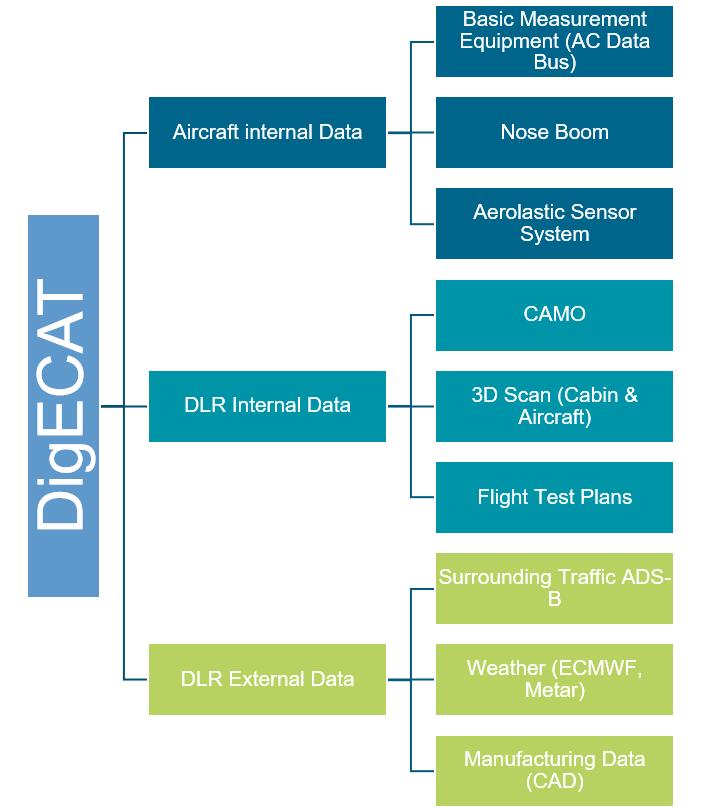
\includegraphics[width=0.48\textwidth]{03_figures/DIGECAT}
    \caption[Components of the Digital Twin]{The different components of the ISTAR Digital Twin. The components not dealt with in this work include the \textit{DLR Internal Data} as well as the \textit{DLR External Data}. The components actually covered in this work include the \textit{Aircraft Internal Data} as previously mentioned in Chapter \ref{chap:meet_the_istar} including the Basic Measurement Equipment as well as the aeroelastic sensor system and the data from the nose boom. \cite{arts_digital_2022}}
    \label{fig:digecat_data_sources}
\end{figure}

\subsubsection{Metadata exchange format}
\label{chap:2-metadata-format}

Aiming for a standardized machine-readable data format the SensOr Interfacing Language (SOIL) is examined. The aircraft data as shown in Figure \ref{fig:digecat_data_sources} is varied in format and shape. For this work however, a data format is needed that is able to handle and represent the intricate details of the aircraft precisely. For the various sources, a metadata enrichment step might be practicable. Effectively, this would act as a metadata importer that fuses metadata and also translates it into SOIL.

%□ DAQ-config □ Aircraft config and parameter info □ Metadata enrichment --> SOIL

\subsubsection{Data Parsing}
Another pillar of this work will be the format the original data is available in. The data the SHM will work on originates from the ISTAR and needs to uploaded without any modification to preserve originality and reduce the room for errors. This small section will deal with the handling of data from the aircraft until it reaches its destination in the Skystash.

Firstly, the Data is uploaded to the stash from the aircraft DAQ format. Its data is available in the proprietary IMC \textit{.raw} formats. These are then parsed into the stash by converting them into timeseries for each parameter. The data structure used in the Skystash is represented in Figure \ref{fig:skystash_data_pipeline}. The folder structure's main path is the project folder which represents the project in which the flight was performed in and contains all the project's flights. Each flight then contains parameter measurements which represent the lowest level of objects in the architecture. All objects of project, flight or measurement type can also contain JSON-usertags as well as additional data in binary format such as pdf files.


%\subsection{Parsing of ISTAR Data}
%ISTAR data originates from the ISTAR's DAQ system in the shape of .raw files for each parameter and is parsed and uploaded to the stash. It is then accessible via the stash api and can also be inspected in the stash webview. After the Dataset generation step the metadata available is only the one from the ISTAR DAQ system.
%The data is present in the shape of Projects->Collections->Series


To provide a full overview of the entire pipeline this step is mentioned. After a flight, the data is stored as a directory full of \textit{.raw} and \textit{.imcexp} files after a flight. Both are proprietary IMC formats with the \textit{.raw} files containing the actual timeseries in an encoded format and the \textit{.imcexp} files then contain the configuration settings for the specific flight or measurement.

The entire directory then gets parsed by a python script. Segmenting the binary structure of the raw files and extracting the timeseries for each parameter. The DAQ and aircraft sensor configuration for each flight gets exported from the imcexp file and uploaded to the Skystash without modification to preserve genuineness of the data as shown in Figure \ref{fig:skystash_data_pipeline}. Any Metadata in shape of a JSON format is represented with a red dot and any binary formats such as pdf files or other custom data are represented with a blue dot.

\begin{figure}
    \centering
    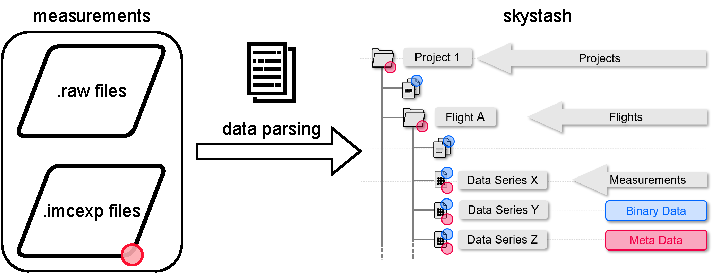
\includegraphics[width=0.8\textwidth]{skystash_data_pipeline}
    \caption[FTI-Microservices: Data Provision]{Pipeline preceding the data provisioning step shown in Figure \ref{fig:SHM_simplified} which consists of parsing the proprietary \textit{.raw} (data) and \textit{.imcexp} (metadata) files provided by the DAQ into a standardized format that is then available in the Skystash. The internal Skystash structure is also shown which consists of three distinct hierarchical levels for research projects which are structured into single flights (recording sessions) which then contain sensor measurements in time-series format. All metadata that exists next to the actual time-series can exist in a JSON-format (shown in red) as well as in an uninterpreted raw format (blue).}
    \label{fig:skystash_data_pipeline}
\end{figure}

Parameters are saved under the flight object. Configuration data is assigned to the user tags of each parameter. The data is then parsed for each flight and inherent sensor. The ISTAR DAQ metadata is currently the only metadata in the Skystash. Since this metadata needs further information to make it understandable it will be enriched further within the Configuration step (See Figure \ref{fig:fti_microservices}).

\subsubsection{Use of FAIR in the implementation}
To now fulfill FAIR principles, the interfaces in the architecture are examined. The generated flight test data is available and metadata is already in a JSON-file format. To further specify and standardize metadata the metadata can be translated into a standardized format to further Interoperability. This enriched metadata then can be fed into the FMEA step. Exiting the FMEA-step, the Analysis results can also be defined within a SOIL/JSON format and then get opened by other applications to access data quality results and perform further analysis steps, increasing reusability.

%Explain which means are taken to guarantee an architecture throughout the work that ensures an implementation of the FAIR principles and the V-model. Architecture of the JSON-Tree structure and which data is inserted where.

By implementing standardized JSON-data structures for the metadata including dataset and report, interoperability as well as reusability are guaranteed. To increase findability, the Skystash architecture is used which generates a unique identifier for every dataset. \cite{meyer_development_2020}. By enriching metadata, findability as well as accessibility is guaranteed. And finally, converting to SI-units guarantees accessible, interoperable and reusable data.

\newpage


\section{SHM results configuration}

Within the last step of the FMEA, the generated report results need to be analyzed which in turn might necessitate change of the FMEA parameters. To facilitate the process and lower the barrier of entry, the possibility of an interactive report respectively dashboard is examined with the ultimate goal to output a report that is clear, concise and standardized.

%\subsection{Challenges}

The requirements for such a report are firstly motivated by necessity. It is vital to show error detection, embed the report into the toolchain and find a format to communicate metadata as well as SHM findings. Such a report tool could then also be used in the development of new algorithms since it generates quick feedback and precise feedback, aiming to display various Indicators for data quality and FMEA quality.


\section{Summary}
In chapter 2 the fundamental definitions for system behavior from the field of control theory have been set forth as standardized descriptors of this work. The theoretical foundation has been created for this work by explaining methods from the field of FMEA and parity equations have been chosen for the further use in this work. Furthermore, the software-side of this work has been introduced. With metadata frameworks and the Skystash platform forming the infrastructure that this work rests on. The learnings from the metadata models within the SOIL infrastructure and the ontology field have been examined and will be implemented in the following. FAIR principles have been presented and have been contextualized within this work. Building upon these fundamentals the next chapter will present an in-depth problem description followed by Chapter \ref{chap:4-methods} presenting the implementation details as well as the implemented methods in this work.



